\chapter{Acceleration-Sensitive Interference}\label{chap:atom_int}

\section{Chapter Outline}
This chapter describes the aspects of the project aimed at observing
matter-wave interference in \ac{rb87} and its subsequent
characterisation. The laser system used to drive the necessary Raman
transitions is presented in~\SectionRef{sec:msquared_laser}. This is
followed by a discussion of the methods used to detect the population
in each internal state in~\SectionRef{sec:atom_detection}. The Raman
transition spectrum and
dynamics of the atoms during each Raman pulse are discussed
in~\SectionRef{sec:atomint_rabiosc}. This chapter continues
with an overview of indentified sources of noise and their impact on
the interferometer's sensitivity to accelerations
in~\SectionRef{sec:atomint_sensitivity}. Finally, a presentation of observed
interference and an analysis of its sensitivity to accelerations is
given in~\SectionRef{sec:atomint_accelerations}.
\section{The M-Squared Laser System}\label{sec:msquared_laser} 
  This section describes the laser system manufactured by \textit{M-Squared
  Lasers}, which is used to drive Raman transitions. 
  A \ac{pll} controls the phase difference of two Ti:Sapphire lasers
  by comparing the beat note with a stable local oscillator\nocite{Lautier2014b}\nocite{Marino2008}. An overview of the laser
  system can be found in~\SectionRef{subsec:msquared_overview}, which includes
  the techniques used to externally communicate with the laser's ICE-BLOC
  control modules. The control of the frequency and phase-lock is then described
  in~\SectionRef{subsec:msquared_control}. Finally, this section concludes
  in~\SectionRef{subsec:dcs_module} with a description of the DCS
  module which is used to control
  the amplitude, frequency and phase of the Raman laser beat-note
  during the experiment.
\subsection{Laser System Overview}
\label{subsec:msquared_overview} The Raman laser system contains two
SolsTiS lasers, each generating \sivalue{780}{\nm} light by pumping a Ti:Sapphire crystal housed inside a resonator.
The output light is frequency-stabilised using piezo-electric stacks to adjust
the resonator length~\cite{Drever1983}. A schematic diagram of this laser system is given
in~\FigureRef{fig:msquared_laser}. Each laser is pumped using a
\sivalue{12}{\W} \textit{Lighthouse Photonics} Sprout laser at
\sivalue{532}{\nm}. One SolsTiS acts as the master frequency locked
to an absorption feature in the saturated absorption spectrum of
\ac{rb87}. The second is slaved to this using a phase-locked loop to keep their
beat frequency constant. The two beams are mixed on a
\ac{pbs}, so that they are orthogonally polarised. Two \acp{aom} control the
output power. 
%A planned upgrade for this system will have multiple output ports
%for the Raman light, which will require independent control. 
\par\noindent 
The system contains 4 ICE-BLOC modules which implement various types of control. The
first two (one for each Solstis) are used to stabilise the output power of each
laser by feeding back to the corresponding Sprout laser. They are also used to
coarsely adjust the output frequency, which is measured using a
\textit{HighFinesse} wavemeter. The third is used for the \ac{pll}
and feeds-back onto the slave laser to control both the frequency and phase of
the optical beat-note between the two lasers. The final ICE-BLOC, referred to
as the DCS module, is used to control the lasers in real-time during the
experiment.  
\begin{figure}
	\centering \fontsize{10pt}{10pt}
	\resizebox{0.8\textwidth}{!}{\input{msquared_laser.pdf_tex}}
	\caption[M-Squared Laser System Schematic]{Schematic Diagram of the M-Squared
		laser system. Two SolsTiS lasers provide the two Raman frequencies, which
		are fibre coupled onto the orthogonal axes of a \ac{pm} fibre. Control of
		the power, frequency and phase as required to drive and control
    the Raman transitions is
		handled by the four ICE-BLOC modules indicated in blue. Further detail of
		this control is given in the text.} \label{fig:msquared_laser}
\end{figure}

\subsubsection{External ICE-BLOC Control}
The ICE-BLOC modules are able to communicate with each other using an Ethernet
hub. Another computer connected to this network is able to control them by
accessing a web page that each module hosts. These web pages control the ICE-BLOCs
by sending structured JSON messages. This graphical interface can be bypassed by
directly communicating these messages. This is done using MOTMaster so that
various parameters, such as the frequency and phase of the Raman beat-note, can
be automatically varied between experiment cycles. 
\subsection{Frequency and Phase Control}\label{subsec:msquared_control}

\subsubsection{Master Lock}
The frequency of the master laser is stabilised using saturated absorption
spectroscopy in a Rubidium vapour cell. Part of the beam is picked off and
modulated by an \ac{eom}. The positive frequency sideband is used to lock the
master laser to the 2,3 crossover feature. In effect, this means that the
modulation frequency of the \ac{eom} sets the one-photon detuning of the Raman
transition. The modulation frequency is set so that the master laser frequency
is \sivalue{1.13}{\giga\hertz} below the \trans{2}{3} transition. This
frequency is chosen because the light shift of the clock transition
vanishes there provided the two Raman beams have the right intensity
ratio as discussed in~\SectionRef{subsec:light_shift}. This ensures
that the resonant frequency is independent of variations in the
over-all intensity of the Raman beams.
\subsubsection{Frequency and Phase Lock} The optical beat-note between the two
lasers is measured using a fast photodiode. The signal from this is used in a
\ac{pll} to fix the relative phase between the two lasers. A frequency
divider halves the frequency of the signal before comparing it to a \ac{vco} of
around \sivalue{3.4}{\giga\hertz}. This creates an error signal which used to
control both the frequency and phase of the beat-note by feeding back to the
slave laser Solstis. The relative phase between the two lasers is adjusted using
an analogue phase shifter and the frequency difference is controlled by tuning
the \ac{vco} frequency. \par\noindent The beat-frequency of the Raman lasers can
be chirped by triggering a ramp of the control voltage to the \ac{vco}. For
chirp rates of lower than \sivalue{24}{\mega\hertz\per\second}, the phase-lock
is able to keep the beat-note phase-coherent during the chirp.  
\subsection{The DCS Module}\label{subsec:dcs_module} 
The DCS module is used to control the
output of the lasers during the experiment. It uses an on-board
\ac{dds} to
synthesise the \sivalue{80}{\mega\hertz} driving frequencies for each \ac{aom}.
The majority of the control is done using an \ac{fpga} that synthesises a timed
sequence of analogue and digital voltage waveforms. An example of a sequence
created using the DCS web interface is shown in~\FigureRef{fig:dcs_module}. The
sequence is segmented into individual steps and each channel can be separately
configured, much like the MOTMaster user interface. \par\noindent This module is
used to control the amplitude, frequency and phase of each Raman pulse. The
pulse amplitude is shaped using an analogue voltage to control the power of the
RF frequency. The voltage output has been calibrated so that the pulse can be shaped to
produce a square, Gaussian or Blackman amplitude envelope. A frequency
chirp of the beat-note is
optionally triggered by sending a digital pulse to the \ac{pll} ICE-BLOC.
\par\noindent The synthesiser can be configured to run continuously, or to wait
at a chosen timestep for an external trigger. It can also iterate through a set
number of parameters, such as timestep duration or phase shift by re-building
the sequence after each cycle.  
\begin{sidewaysfigure}[!htbp] 
  \centering
	\resizebox{1\textwidth}{!}{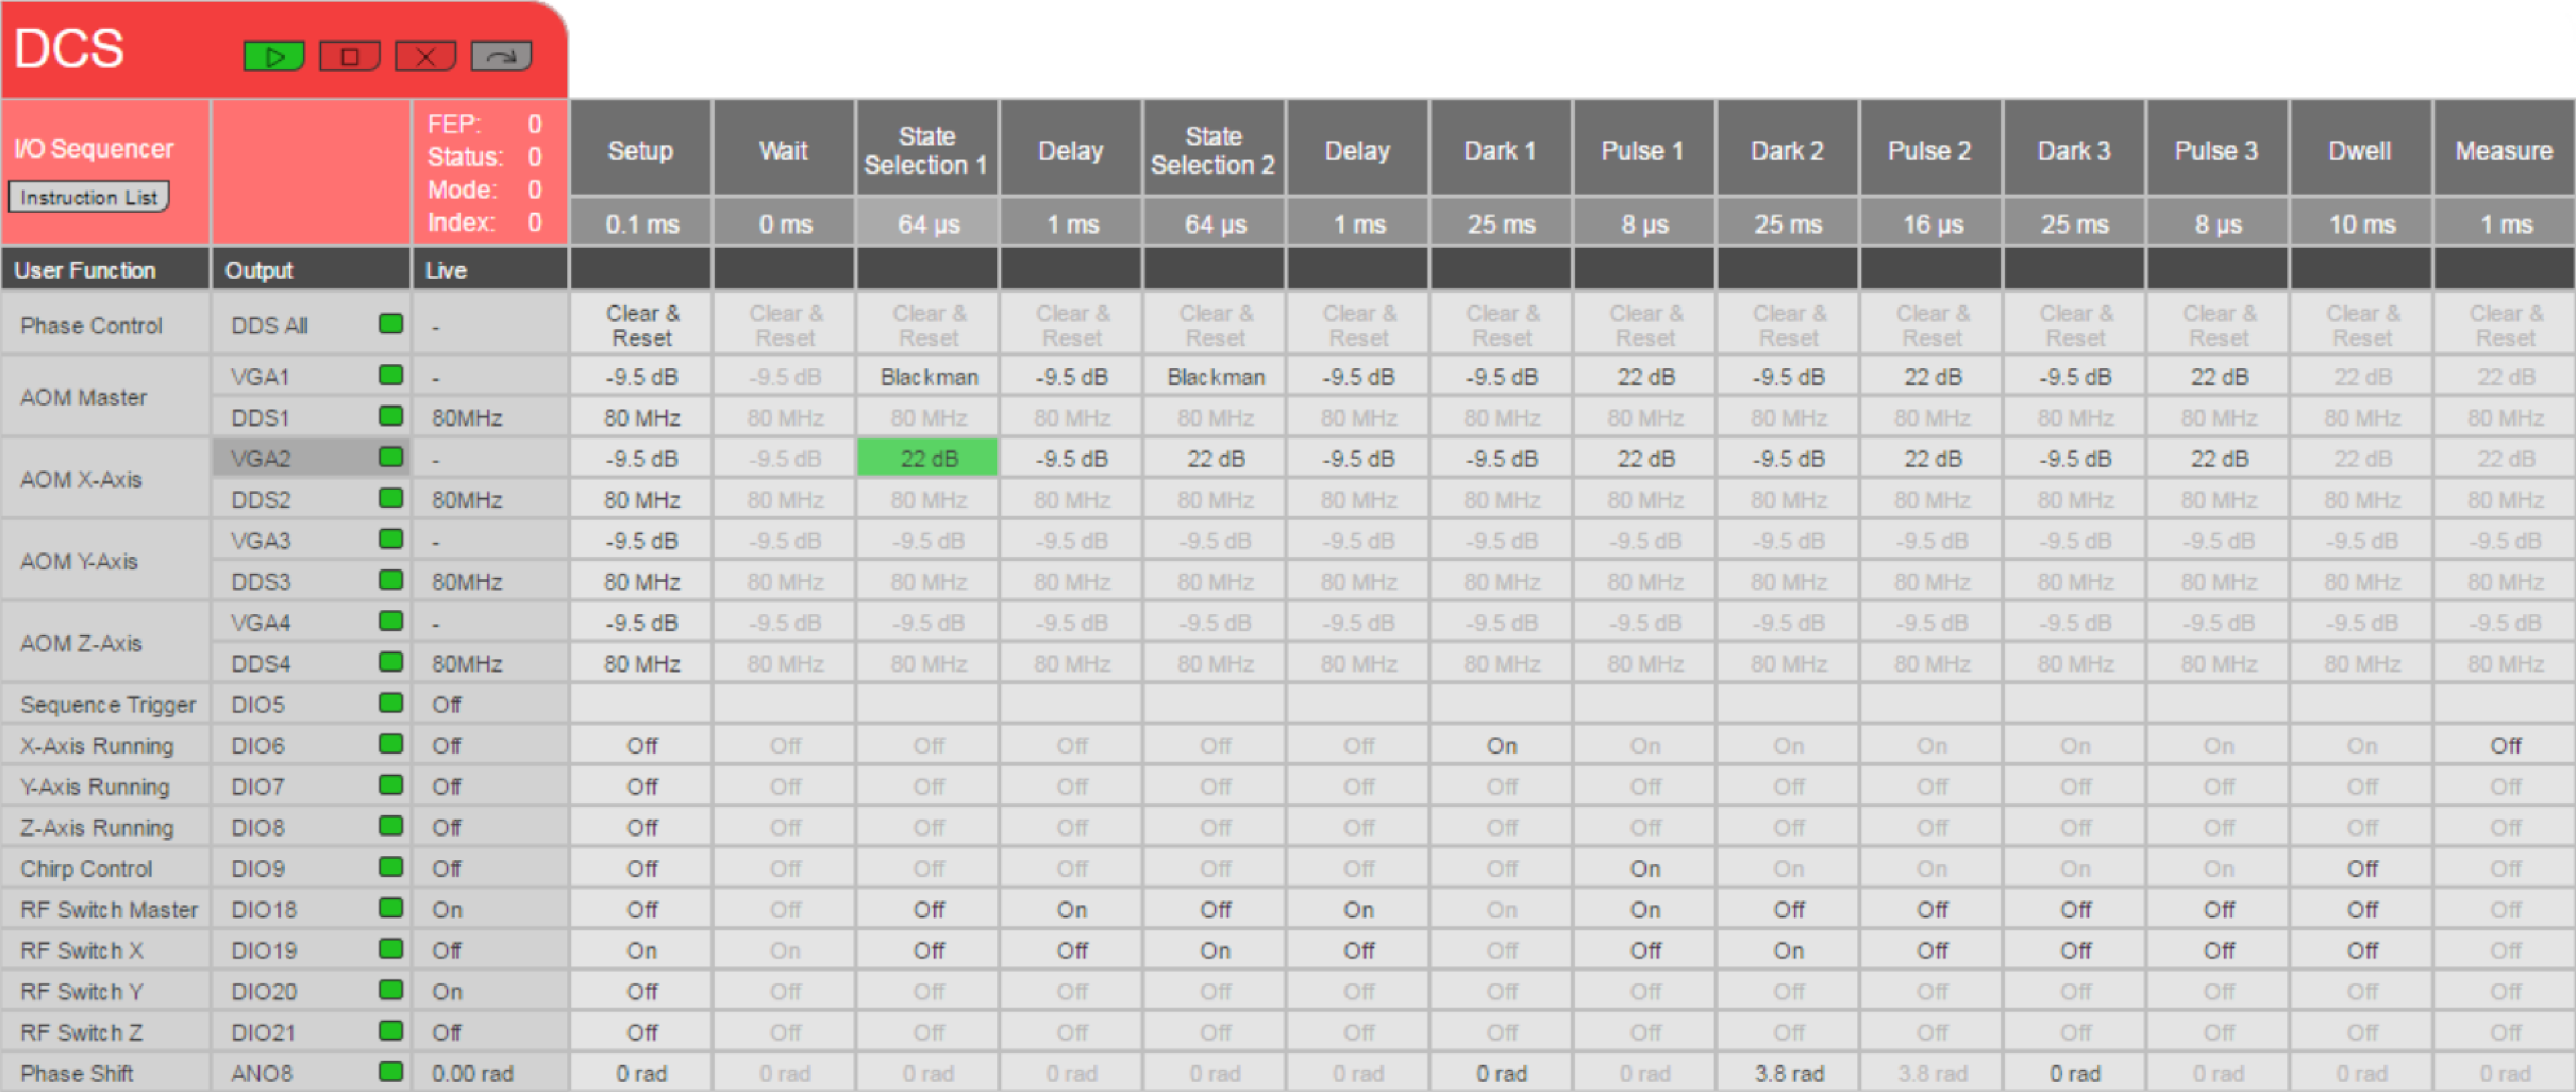
\includegraphics{dcs_module.pdf}}
	\caption[DCS Module User interface]{DCS module user interface. The sequence is
		synthesised from individual steps. The parameters of each Raman laser pulse
		can be configured independently.} 
  \label{fig:dcs_module} 
\end{sidewaysfigure}
\section{Atom Detection}\label{sec:atom_detection} 
This section describes the methods used to
measure the number of atoms in each hyperfine ground state and infer
the interferometer phase. It begins with a
presentation the optical setup used to collect fluorescent light on a
photodiode in~\SectionRef{subsec:optical_setup}.
The scheme used to detect the atoms by
driving \(\sigma^+\) transitions is then described in~\SectionRef{subsec:optical_setup}.
This concludes with a
discussion on converting the measured photodiode signals into atom
number and interferometer phase
in~\SectionRef{subsec:phase_measurement}.
\subsection{Optical Setup}\label{subsec:optical_setup}
Out aim in this device is to reach the standard quantum noise limit,
which comes from the quantum projection noise. Expressed as a
fractional accuracy this is given approximately by
$N^{-1/2}$~\cite{Bollinger1996}, where $N$ is the number of atoms detected.
The CCD used initially was not sensitive enough for this as there wass a
significant amount of noise in reading out the charge collected at each pixel.
Instead, a more sensitive photodiode is used to detect the atoms. With a
suitably high bandwidth, the readout time is much faster than the CCD as well,
so that the atoms can be detected well before they fall out of the field of
view. \par\noindent A diagram of the setup used to detect the atoms is given
in~\FigureRef{fig:photodiode_optics}. It is a triplet system which uses
lenses with focal lengths \sivalue{150}{\milli\metre},
\sivalue{75}{\milli\metre} and \sivalue{60}{\milli\metre}, with the
\sivalue{150}{\mm} lens closest to the atoms and the \sivalue{60}{\mm}
lens closest to the photodiode. A ray-tracing simulation of the optical
system indicates spherical aberrations on the image. This is caused by
the third lens, which was added to shorten the back focal length. The
front lens has a diameter of
\sivalue{50.4}{\milli\metre}, so the solid angle subtended by the
optics is \(4\pi \times\)\num{7.1e-3}\si{\steradian}.
\begin{figure}[!htbp] 
  \centering \fontsize{24pt}{24pt}
	\resizebox{0.7\textwidth}{!}{\input{photodiode_optics.pdf_tex}}
	\caption[Optical setup for Photodiode Detection]{Optical setup for photodiode
		detection. A triplet lens system focuses light from radiated from the atoms
		onto a photodiode. This is mounted using a translation stage to
  position the photodiode at the back focal point.}
  \label{fig:photodiode_optics}
\end{figure}

\subsubsection{Photodiode Calibration}
The photodiode used is a \textit{Femto LCA-S-400K-SI},
which has a trans-impedance amplifier with a bandwidth of \sivalue{400}{\kilo\hertz} and a photo-sensitive area
with a diameter of \sivalue{3}{\milli\metre}. The scaling factor from
incident optical power to output voltage was measured as \sivalue{1.84e6}{\volt\per\watt}. 
%\begin{figure}[htpb]
%  \centering
%  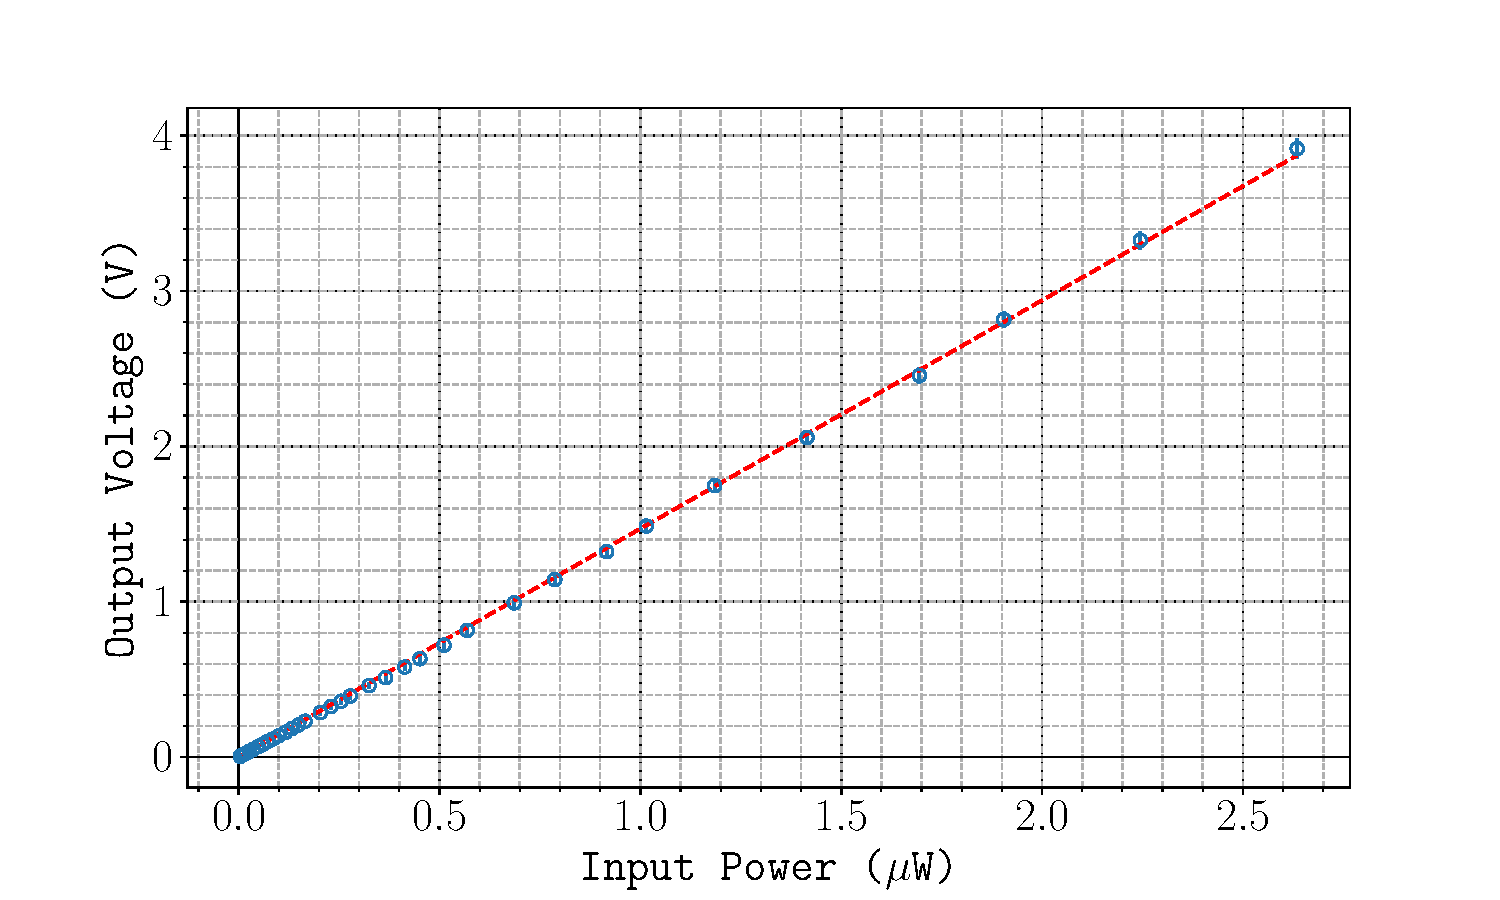
\includegraphics[width=0.8\linewidth]{Figures/Chapter6/pd_calib.pdf}
%  \caption{Name}
%  \label{fig:name}
%\end{figure}
\subsection{Detection using \(\sigma^+\) transitions}\label{subsec:photodiode_setup}
The atoms are detected using resonance fluorescence from the two
vertically aligned \ac{mot} beams in the presence of a vertical
magnetic field. For the \ac{mot} and molasses these are polarised
$\sigma^+$ and $\sigma^-$, but for this detection step, we use a
liquid-crystal \ac{hwp} to give both beams $\sigma^+$ polarisation.
This causes the atoms to be optically pumped into \(\ket{2,2}\) and cycle on the
\(\ket{2,2} \rightarrow \ket{3,3}\) transition, which allows the atoms
to scatter many photons with minimum probability of unwanted optical
pumping into $\ket{F=1}$.
\par\noindent
\FigureRef{fig:detection_scheme} shows the setup used to invert the
polarisation of one \ac{mot} beam prior to detection. The liquid-crystal
waveplate is an electro-optical device whose birefringence changes
when an ac voltage is applied across it. The waveplate is placed at
the output of the downward-propagating (\(\vec{z}_-\))
collimator. The liquid-crystal waveplate is triggered to rotate the
incoming linearly polarised light by $\pi/2$ \sivalue{}{\radian}. 
\begin{figure}[!htpb]
    \centering
    \fontsize{14pt}{14pt}
    \resizebox{0.5\textwidth}{!}{\input{detection_scheme.pdf_tex}}
    \caption[Scheme to invert beam polarisation.]{Scheme to invert
      beam polarisation. In the \ac{mot} loading phase of the
      experiment, the liquid crystal \ac{hwp} is oriented to give a
      right-hand circular polarised beam shown in blue. Prior to
      detection, a digital pulse triggers a re-orientation of its slow
      axis. This results in a left-hand circular polarised beam, shown
      in red.}\label{fig:detection_scheme}
\end{figure}
\subsubsection{Detection Sequence}\label{subsec:detection_sequence}
The sequence used to detect the atoms is shown
in~\FigureRef{fig:detection}. Shortly before the sequence starts, the
bias field is aligned to the \(\vec{z}\) axis and the liquid-crystal
waveplate is triggered to change the handedness of the \(\vec{z}_-\)
beam. The cooling laser frequency is set so it is detuned by
\(\delta_D =\) \sivalue{3}{\mega\hertz}
below the \trans{2}{3} transition and the repump laser is set to
resonance with the \trans{1}{2} transition. This creates an optical
molasses which avoids heating the atoms so that they remain in the
detection volume for a longer period of time. The intensity of the
light is reduced to around \(3 I_\text{sat}\). As shown below, this
intensity was empirically found to minimise the variance in output
voltage. The acquisition of the photodiode voltage is
triggered to start at the first Dwell time. Durin The cooling light is first
switched on without any repump light so that only atoms in \(\ket{F=2}\) scatter light. After this, the repump
is switched on, so that atoms in \(\ket{F=1}\) are optically pumped
into \(\ket{F=2}\) and all the atoms scatter light. Now the
fluorescence measures the total number of atoms $N$. This repump light is a
sideband of the cooling laser, so the total output is increased
to ensure that the intensity of the cooling light remains constant.
Each detection step lasts \sivalue{250}{\micro\second}, but the
first \sivalue{50}{\micro\second} is discarded to allow time for the
intensity to stabilise and for optical pumping into \(\ket{F=2}\).
All the atoms are then blown away by switching off one of the detection
beams before the sequence is repeated to collect a
background signal.
\begin{figure}[!htbp] 
  \centering
  \fontsize{14pt}{14pt}
  \resizebox{0.8\textwidth}{!}{\input{detection.pdf_tex}} 
  \caption[State detection sequence timing]{Timing diagram for state
    detection. Atoms in \(\ket{F=2}\) are detected first, then repump
    light pumps the \(\ket{F=1}\) atoms into $\ket{F=2}$ so they are detected as well. A
background light measurement follows the measurement of the atom
numbers.}
	\label{fig:detection} 
\end{figure}
\subsubsection{Maximum Detection Time}\label{subsubsec:intensity_dependendce}
As the atoms scatter light during detection, the cloud will be heated
and expand due to the momentum exchanged from absorption and
spontaneous emission. The atoms are only cooled along the axis of the
detection beams, so the heating rate is greatest along the other two
axes. It is necessary to ensure that the
heating rate is low enough that the atoms remain within the
detection beam for the entire detection time. A requirement on the
maximum detection time can be obtained as follows. The momentum of
an atom scattering photons follows a random walk, so 
if the cloud has a
Gaussian spatial distribution with an
initial width of \(\sigma_0\), the width at a later time of
is given by
\begin{equation}
\sigma_x^2(t) = \sigma_0^2 + \frac{2 n_p v_r^2 t^2}{3} 
  \label{eq:width_scattering}
\end{equation}
where \(v_r = \frac{\hbar k}{m_\text{rb}} =
\) \sivalue{6}{\milli\metre\per\second} is the recoil velocity and \(n_p\) is the
number of photons scattered. The factor of $2/3$ is because only the
transverse component of the recoil is relevant here. To remain within the detection region,
the width of the cloud must be smaller than the detection beam waist
\(w\), so the detection time must satisfy
\begin{equation}
  t_D \ll \sqrt{\frac{3 \left(w^2-\sigma_0^2\right)}{2 \left(n
  v_r^2\right)}}
  \label{eq:detection_time}
\end{equation}
For a beam waist of \sivalue{7.5}{\milli\metre}, initial cloud size of
\sivalue{5}{\milli\metre} and a maximum scattering rate of
\sivalue{2e7}{\per\second} the detection time must be much less than
\sivalue{4.7}{\milli\second}. This inequality is amply satisfied by
our detection time of \sivalue{100}{\micro\s}.
%\begin{equation}
%  p(x,t) = \int \frac{1}{\sqrt{2\pi} e^{-\frac{(x + \frac{p}{m}
%    t)^2}}{2 \sigma_x^2} \frac{1}{\sqrt{2\pi D t} e^{-\frac{p^2}{2 D
%      t}} \mathrm{d}t
%  \label{eq:prob_atom_diff}
%\end{equation}
\subsubsection{Detection Intensity}
The intensity for detection was chosen by varying the total power
in the detection beams and recording the photodiode voltage for a
fixed detection time of \sivalue{200}{\micro\second}.
\FigureRef{fig:photodiode_intensity_calib} shows the average voltage
measured when detecting atoms in the \(\ket{F=2}\) state as the
intensity of the light increases. The saturation parameter \(s\) is
inferred from the control voltage used control the light
through the \ac{aom} at the output of the
\Muquans laser (see~\FigureRef{fig:muquans_cooling}) and the peak
intensity of the \ac{mot} beams. By the time the atoms are detected,
they have moved away from the region of peak intensity, so the
intensity on the atoms is smaller than the applied control voltage
would indicate if they were at the peak intensity. A fit parameter $b$
is introduced to account for this. A non-linear least squares fit
to the function
\begin{equation}
  v = a\frac{b s}{1 + b s + 4 \left(\delta_D/\Gamma\right)^2}
  \label{eq:voltage_fit}
\end{equation}
gives a scaling for the intensity of \(b = 0.83\). The variance in the
measured voltage (for a constant mean number of atoms) is minimised when the
intensity is around 3\(I_\text{sat}\). Above this intensity, there is
a significant depopulation into \(\ket{F=1}\) caused by off-resonant
excitations to the \(\ket{F'=2}\) state.
This is evident in the voltage signal over time, which is
shown in \FigureRef{fig:detection_time} for various intensities. At an
intensity of 3\(I_\text{sat}\), around 5\% of the population is
pumped out of \(\ket{F=2}\).
\begin{figure}[htpb!]
  \centering
  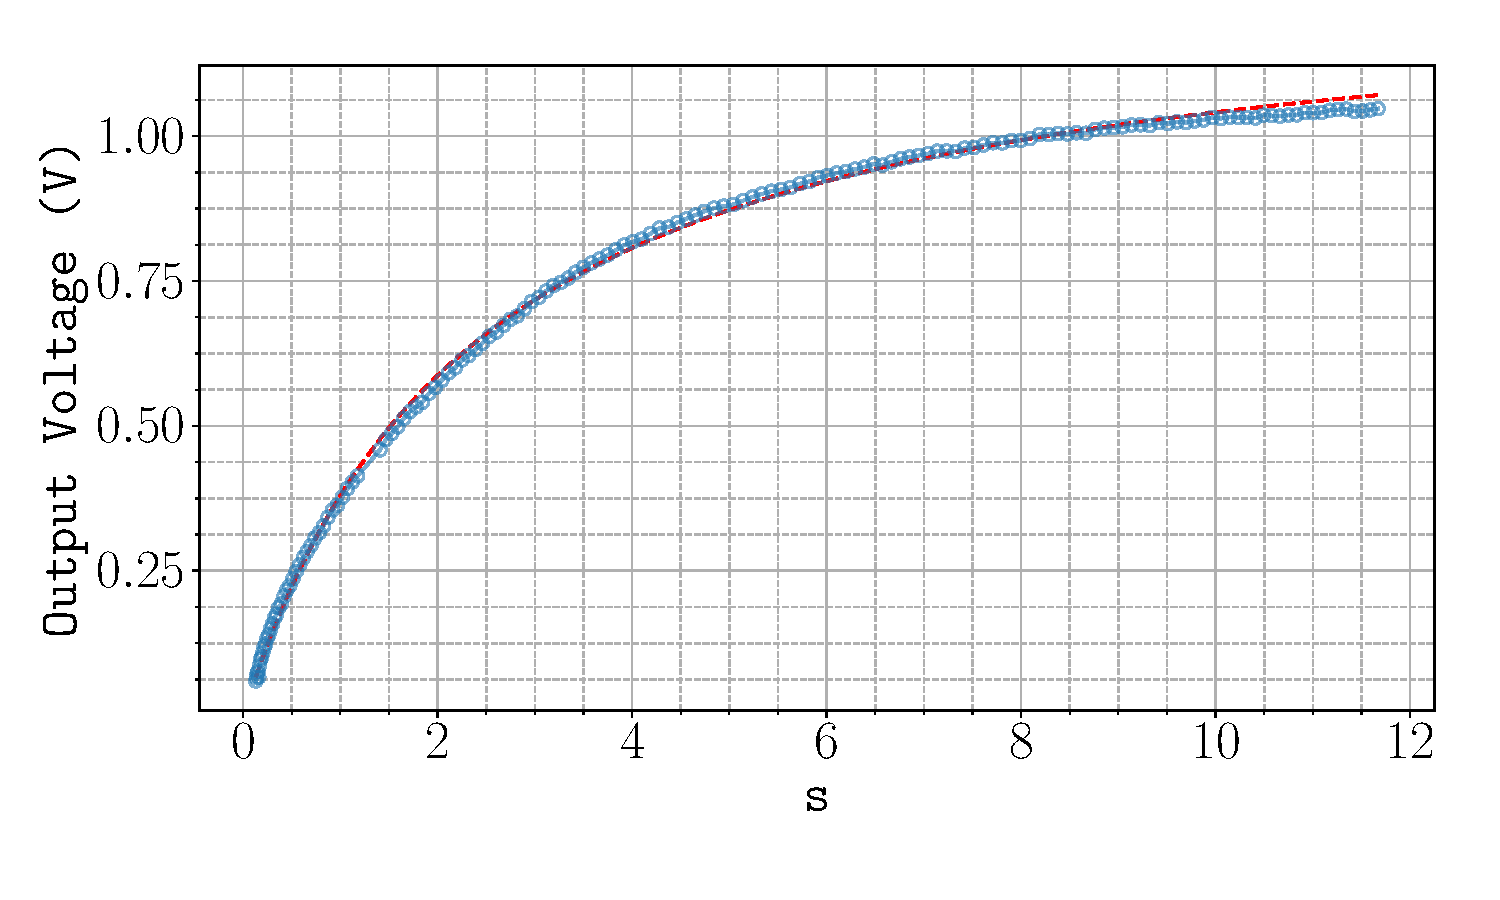
\includegraphics[width=0.7\textwidth]{photodiode_intensity}
  \caption[Photodiode output voltage for increasing detection beam
  intensity. ]{Photodiode output voltage for increasing detection beam
  intensity. The red dashed line indicates a fit
to~\EquationRef{eq:voltage_fit} to estimate the scaling factor for the
saturation parameter \(s\).}
  \label{fig:photodiode_intensity_calib}
\end{figure}

\begin{figure}[htpb!]
  \centering
  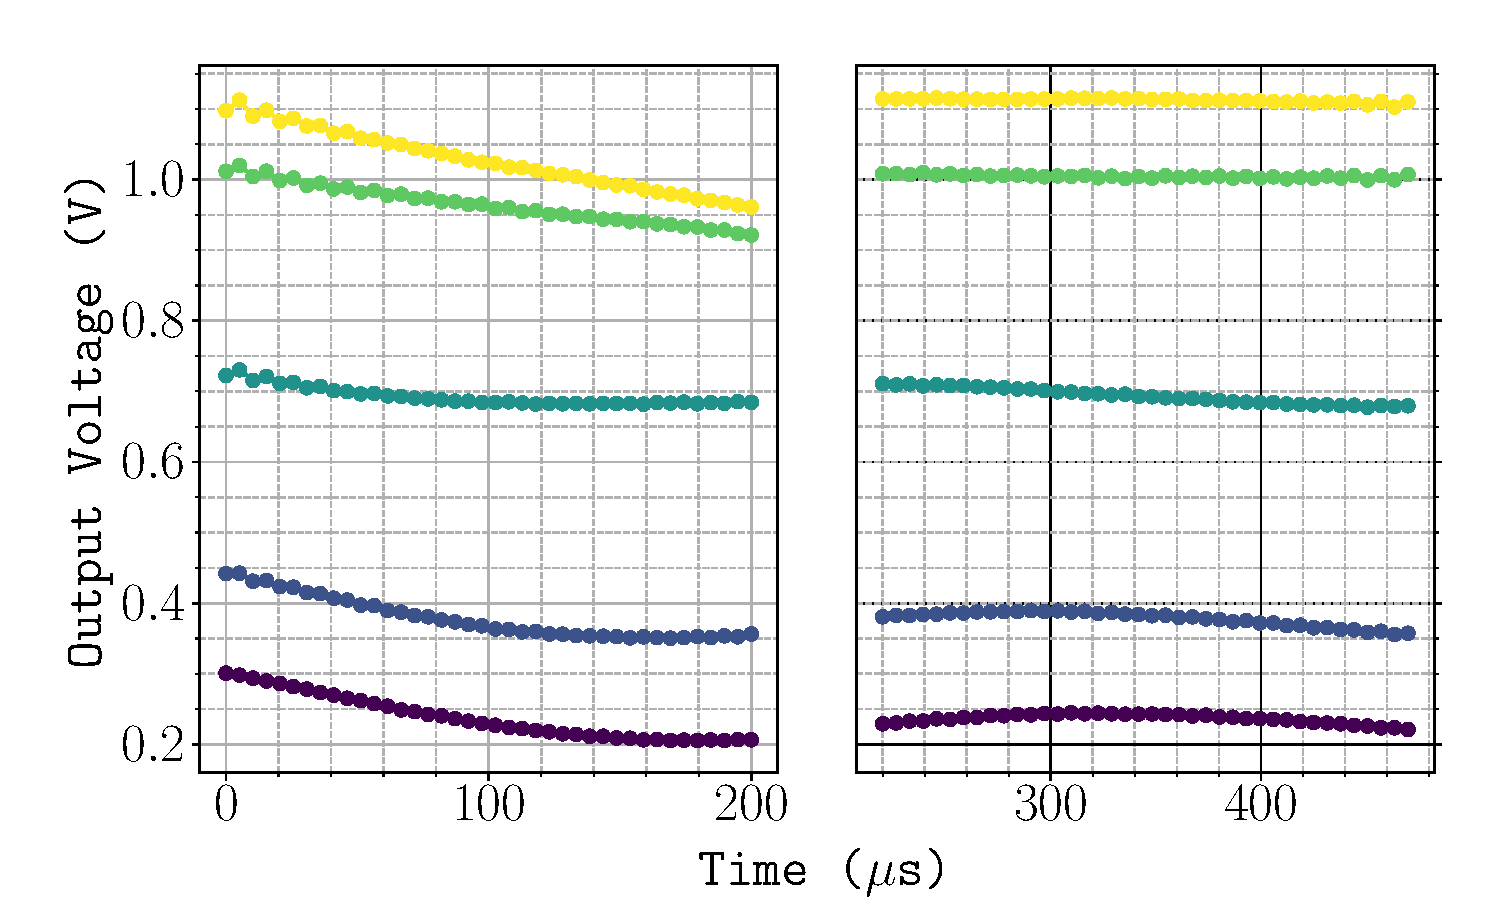
\includegraphics[width=0.7\textwidth]{photodiode_voltage_time}
  \caption[Photodiode voltage for varying detection times.]{Photodiode voltage over time during detection for \(s =
    0.5, 1, 3, 7, 10\) in order from purple to yellow.}
  \label{fig:detection_time}
\end{figure}

\subsection{Measuring the Occupation Probability}\label{subsec:phase_measurement}

The occupation probability of the $\ket{F=2}$ state is obtained by measuring the proportion of
atoms in each hyperfine ground state. The voltage of the amplified
photodiode signal is related to the number of atoms
\(n_\text{at}\) that scatter light on the cycling transition by
\begin{equation}
 V &= \eta R_\text{sc}(s,\delta) n_\text{at} \hbar \omega G 
  \label{eq:pd_signal}
\end{equation}
where \(\eta = \Omega/4\pi\) is the fractional solid angle subtended by the
collection optics, \(\hbar\omega = \sivalue{1.6}{\electronvolt}\) is
the photon energy, \(R_\text{sc}\) is the scattering rate per atom defined
in~\EquationRef{eq:scattering_rate} and \(G\) is the photodiode
conversion gain of \sivalue{1.84e6}{\V\per\W}. At the saturation intensity and a detuning of
\sivalue{3}{\mega\hertz}, the voltage measured per
atom is around \sivalue{30}{\nano\volt} per atom. With a detection
time of \sivalue{200}{\micro\s}, around 7 photons per atom are
detected. The probability of
an atom occupying \(\ket{F=2}\) is estimated as follows
\begin{equation}
  \text{P}_{\ket{F=2}} =
  \frac{\text{N}_2}{\text{N}_\text{Tot}}
  \label{eq:prob_measurement}
\end{equation}
Here the subscript 2 indicates the average voltage measured with
cooling light only (detecting $\ket{F=2}$ atoms) while the subscript
Tot indicates the average voltage with the repump light as well
(detecting all the atoms). 
The interferometer phase difference \(\Delta\Phi\) is determined from \EquationRef{eq:prob_measurement} using
\begin{equation}
  \text{P}_{\ket{F=2}} = \text{P}_0 - \frac{C}{2}\cos(\Delta\Phi)
  \label{eq:interferometer_phase}
\end{equation}
where P\(_0\) is the mean probability of detecting atoms in
\(\ket{F=2}\) and \(C\) is the interferometer fringe contrast. These
are experimentally determined by varying $\Delta\Phi$ as described
in~\SectionRef{sec:fringe_cal}.

\subsubsection{Atom Number Bias}\label{subsec:atom_number_bias}
After the initial state preparation is complete, there are still some
residual atoms left in the states $\ket{F=1, m_F = \pm 1}$. Also, as
shown in~\FigureRef{fig:detection_time}, the photodiode signal that
yields $N_2$ is not constant because some of the $\ket{F=2}$ atoms are
optically pumped into the $\ket{F=1}$ state. In the following, we
consider how both these defects affect the validity
of~\EquationRef{eq:interferometer_phase}.
\par\noindent
If atoms are pumped out of
\(\ket{F=2}\) at a rate \(\gamma\), then the number of atoms in the
number of atoms in $\ket{F=2}$ is given by
\begin{equation}
  n_2(t) = n_{20}e^{-\gamma t}
  \label{eq:n2_time}
\end{equation}
where \(n_{20}\) is the initial number in \(\ket{F=2}\). After
averaging over a time \(\tau\), this gives
\begin{equation}
  N_2 = \frac{n_{20} (1-e^{-\gamma \tau})}{\gamma \tau}
  \label{eq:n2_avg}
\end{equation}
The total number of atoms, measured during the second detection pulse
is
\begin{equation}
  N_\textnormal{Tot} =  n_{10} + n_{20} + n_{\pm 1}
  \label{eq:n1_avg}
\end{equation}
where \(n_{\pm 1}\) is the background population in
\(\ket{1,\pm{1}}\) and $n_{10}$ is the initial population in
$\ket{1,0}$. The detected probability is then
\begin{align}
  \text{P} &= \frac{N_2}{N_\text{Tot}} \nonumber \\
    &= \frac{\frac{n_{20} (1-e^{-\gamma \tau})}{\gamma \tau}}{n_{10} +
    n_{20} + n_{\pm 1}}
    \label{eq:prob_bias}
\end{align}
which is not the same as occupation probability from the
interferometer fringe
\begin{equation}
  \text{P}_0 = \frac{n_{20}}{n_{10} + n_{20}}
\end{equation}
Dividing~\EquationRef{eq:prob_bias} by $n_{10}+n_{20}$, the detected
probability is expressed in terms of $\text{P}_0$ as
follows 
\begin{equation}
  \text{P} = \frac{\text{P}_0}{1+\epsilon}\frac{1-e^{-\gamma \tau}}{\gamma \tau}
\end{equation}
where \(\epsilon = \frac{n_{\pm{1}}}{n_1+n_2}\) is the ratio of the
number of residual atoms to the number in the interferometer.
Similarly, the contrast $C$ of the detected fringe is related to the
actual contrast $C_0$ by 
\begin{equation}
  C = \frac{C_0}{1+\epsilon}\frac{1-e^{-\gamma \tau}}{\gamma \tau}
  \label{eq:contrast}
\end{equation}
For small $\gamma \tau$, this multiplicative factor is
well-approximated by $\frac{1-\gamma \tau}{1+\epsilon}$. 
From~\FigureRef{fig:detection_time}, around 7\% of the signal is lost
for \(s = 3\), so $\gamma = $ \sivalue{360}{\per\s} and $\tau =$
\sivalue{200}{\micro\s}. From the imperfect state preparation, after
velocity selection there is roughly equal population in the $m_F = 0$
state as the $m_F = \pm 1$ states, so we assume $\epsilon = 1$. 
Now the detected contrast is $C = 0.46 C_0$, which includes a factor
of $1/2$ from the $m_F = \pm 1$ atoms. This background population
greatly reduces the detected fringe contrast. Increasing the purity of
the state prior to interferometry will certainly be required to
improve this fringe contrast. 
\section{Individual Pulse Characterisation} \label{sec:atomint_rabiosc}
This section presents a characterisation of the pulses used to drive
Raman transitions between the two hyperfine ground states. First, the
properties of the Raman transition spectrum are presented
in~\SectionRef{subsec:raman_spec}. Following this, a discussion of
cancelling the systematic phase from a differential ac Stark Shift is
given in~\SectionRef{subsec:light_shift}. Finally, this section
concludes with specific details about the individual pulses used in
the experiment. The first Raman pulse, which is used to select a
subset of atoms with a narrow velocity spread, is presented
in~\SectionRef{subsec:vel_select}. This section concludes with a presentation
of the dynamics of the three pulses used to coherently control the
atoms during the interferometer in~\SectionRef{subsec:int_pulses}
\subsection{Raman Transition Spectrum}\label{subsec:raman_spec}
When a circularly polarised light beam excites an atom, the angular
momentum of the light is transferred to the atom. Therefore, a
$\sigma^+$ circularly polarised beam raises the $m_F$ quantum number
by 1 when a photon is absorbed. Similarly, the stimulated emission
induced by a $\sigma^+$ beam lowers $m_F$ by 1. In the case of our
Raman transitions, one beam (with wavevector $\textbf{k}_1$) excites
the atom and another (wavevector $\textbf{k}_2$) stimulates it back
down to the other hyperfine ground state.
\TableRef{tab:raman_polarisation} shows the polarisation selection
rules for these transitions.
\par\noindent
\FigureRef{fig:raman_spectrum} shows an example of the Raman
transition spectrum taken with atoms that have been launched along the
Raman axis at about \sivalue{8}{\cm\per\s}. The beat frequency
between the two Raman lasers is scanned and the light is pulsed for
\sivalue{160}{\micro\second} to drive atoms from $\ket{1,0}$ into the \(\ket{F=2}\)
state. The labels in~\FigureRef{fig:raman_spectrum} indicate the
initial and final $m_F$ values. There is a large narrow peak labelled
$0\rightarrow0$ close to the hyperfine splitting
frequency. This is a result of velocity-insensitive co-propagating
transitions\footnote{When the two light fields are co-propagating, the
  Doppler shift, being proportional to \(\vec{k}_1 -
  \vec{k}_2\) is close to zero}. Looking at the entry
  in~\TableRef{tab:raman_polarisation} for $\Delta m = 0$, this peak
  indicates that the co-propagating beams do not have exactly the
  $\sigma^+ - \sigma^+$ polarisation that was intended. This is further supported by the fact
that there are \(\Delta m = \pm 1\) transitions, which can only occur
if one of the lasers drives a \(\pi\) transition. The Zeeman shifts on
the co-propagating transitions between \(\ket{F=1,0}
\rightarrow \ket{F=2,1}\) and \(\ket{F=1,1}\rightarrow \ket{F=2,1}\)
are \sivalue{95}{\kilo\hertz} and \sivalue{189.5}{\kilo\hertz}, and
are perfectly consistent with the known applied magnetic field of \sivalue{1.4}{\gauss}.
%\begin{table}
%  \centering
%  \begin{tabular}{ccccc}
%    \toprule
%    & & \multicolumn{3}{c}{\(\vec{k}_2\)} \\
%     \midrule
%     & & \(\sigma^-\) & \(\pi\) & \(\sigma^+\)\\
%     \multirow{3}{*}{\(\vec{k}_1\)} & \(\sigma^-\) &  c\(_1\) &
%     c\(_2\)&
%     --  \\
%     & \(\pi\) &c\(_3\) & -- & c\(_4\) \\
%     & \(\sigma^+\) & --& c\(_5\)& c\(_6\)\\
%    \bottomrule
%  \end{tabular}
%  \caption[Raman transition polarisation configurations]{Labels for Raman transitions excited
%    from \(\ket{F=1}\) by \(\vec{k}_1\) and stimulated into
%  \(\ket{F=2}\) by \(\vec{k}_2\).}
%  \label{tab:raman_polarisation}
%\end{table}
\begin{table}
  \centering
  \begin{tabular}{ccccccc}
    \toprule
     & & \multicolumn{5}{c}{\(\ket{F=2,m}\)} \\
     \midrule
     & & -2 & -1 & 0 & 1 & 2 \\
     \multirow{3}{*}{\(\ket{F=1,m}\)} & -1 & (c\(_2\),c\(_4\)) &
     (c\(_1\),c\(_6\)) &(c\(_3\),c\(_6\))& -- & --  \\
     & 0 &-- & (c\(_2\),c\(_4\))& (c\(_1\),c\(_6\)) & (c\(_3\),c\(_6\))
     &-- \\
     & 1 & --& --&(c\(_2\),c\(_4\))& (c\(_1\),c\(_6\)) & (c\(_3\),c\(_6\)) \\
    \bottomrule
  \end{tabular}
  \caption{Allowed polarisation configurations between each hyperfine
  ground state Zeeman sub-levels.}
  \label{tab:raman_polarisation}
\end{table}
\begin{figure}[htpb]
  \centering
  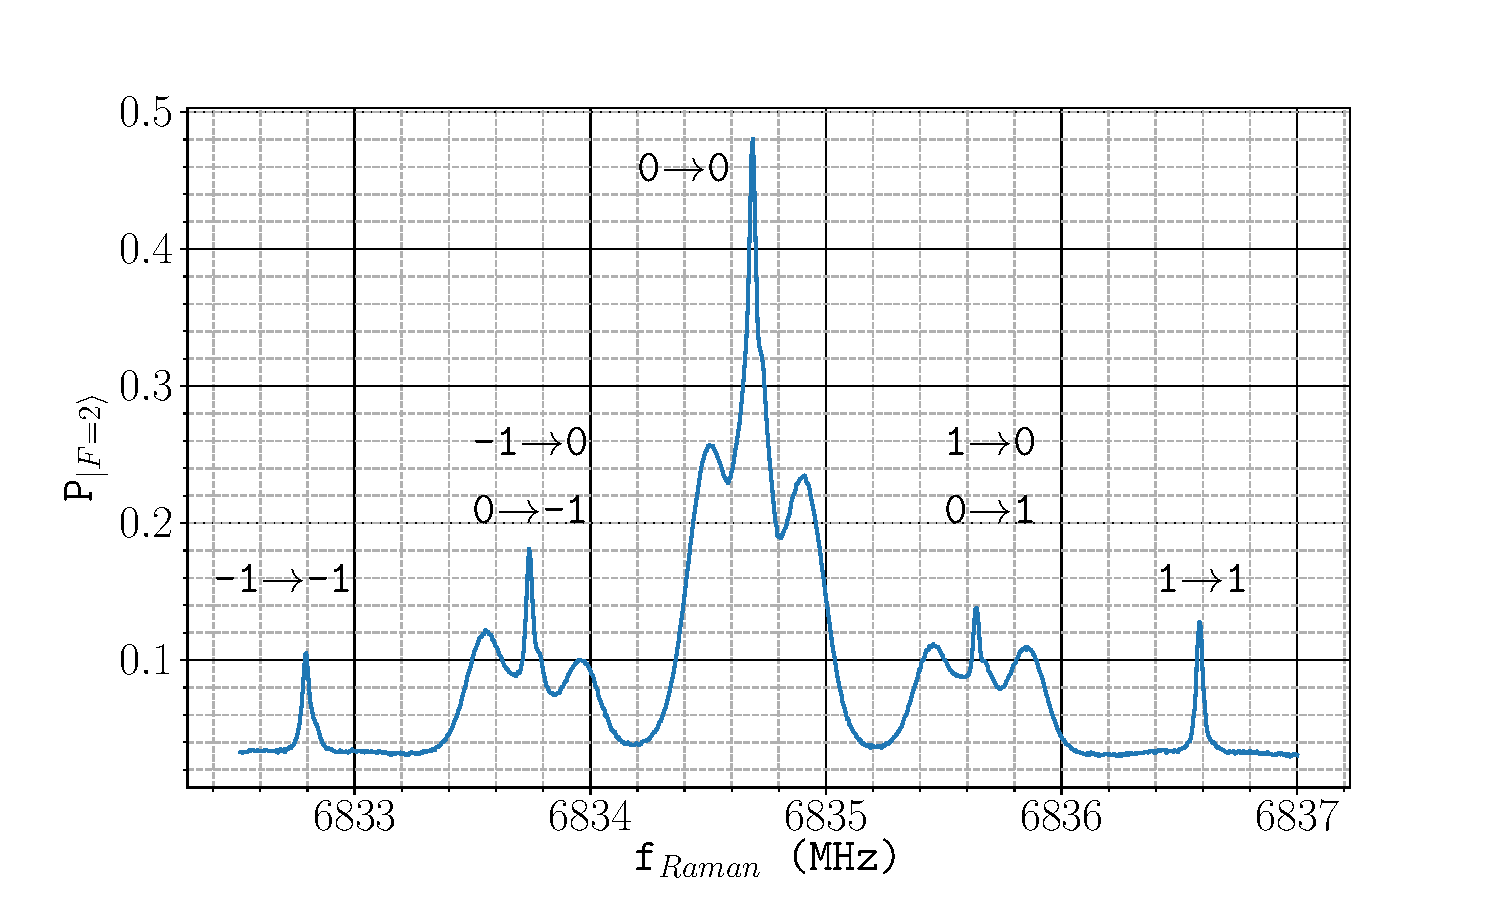
\includegraphics[width=0.7\textwidth]{raman_spectrum}
  \caption[Raman transition spectrum]{Raman transition spectrum, obtained by scanning the beat
    frequency of the two Raman lasers. The transitions \(\ket{1,m_F}
  \rightarrow \ket{2,m_F'}\) are indicated at each observed peak.}
  \label{fig:raman_spectrum}
\end{figure}
\par\noindent
Each narrow transition from \(\ket{1,0}\) has broader
peaks on either side which are the Doppler-sensitive transitions
produced by counter-propagating beams.
The central peak is shown in more detail
in~\FigureRef{fig:raman_spectrum_inset}. The counter-propagating
transitions are shifted from the central co-propagating peak by \sivalue{-185}{\kilo\hertz} and
\(+\)\sivalue{215}{\kilo\hertz} respectively. This difference is
explained by the recoil shift $\Delta f_r = \frac{1}{2\pi}\frac{\hbar
k^2_\textnormal{eff}}{2m} = $ \sivalue{14.9}{\kHz}, which increases
the resonance frequency of both counter-propagating transitions.
After subtracting the recoil shift, the Doppler shifts of
$\pm$\sivalue{200}{\kHz} corresponding to
velocity of \sivalue{7.69}{\centi\metre\per\second}. The same Doppler shifts are also
observed in the peaks corresponding to the \(\ket{F=1,m_F = 0}
\rightarrow \ket{F=2,m_F=\pm 1}\) transitions. The counter-propagating transitions are
Doppler-broadened by the thermal velocity of the atoms along the direction
of the Raman beams. 
%The Doppler shift $\Delta f = \frac{2
%v}{\lambda}$, where $\lambda = $ \sivalue{780}{\nm} broadens the
%transition so that the FWHM is given by
%\begin{equation}
%  \Delta f_\text{FWHM} = 4 \sqrt{2 \ln{2}} \sqrt{\frac{k_B T}{m
%  \lambda^2}}
%\end{equation}
Fitting the transition to the lineshape expected
from a thermal distribution of atoms gives a temperature of
\sivalue{15}{\micro\kelvin} and \sivalue{13.5}{\micro\kelvin} from
each counter-propagating transition. At the time this spectrum was
measured, the molasses was not optimised to give the lowest
temperature.
\begin{figure}[htpb!]
  \centering
  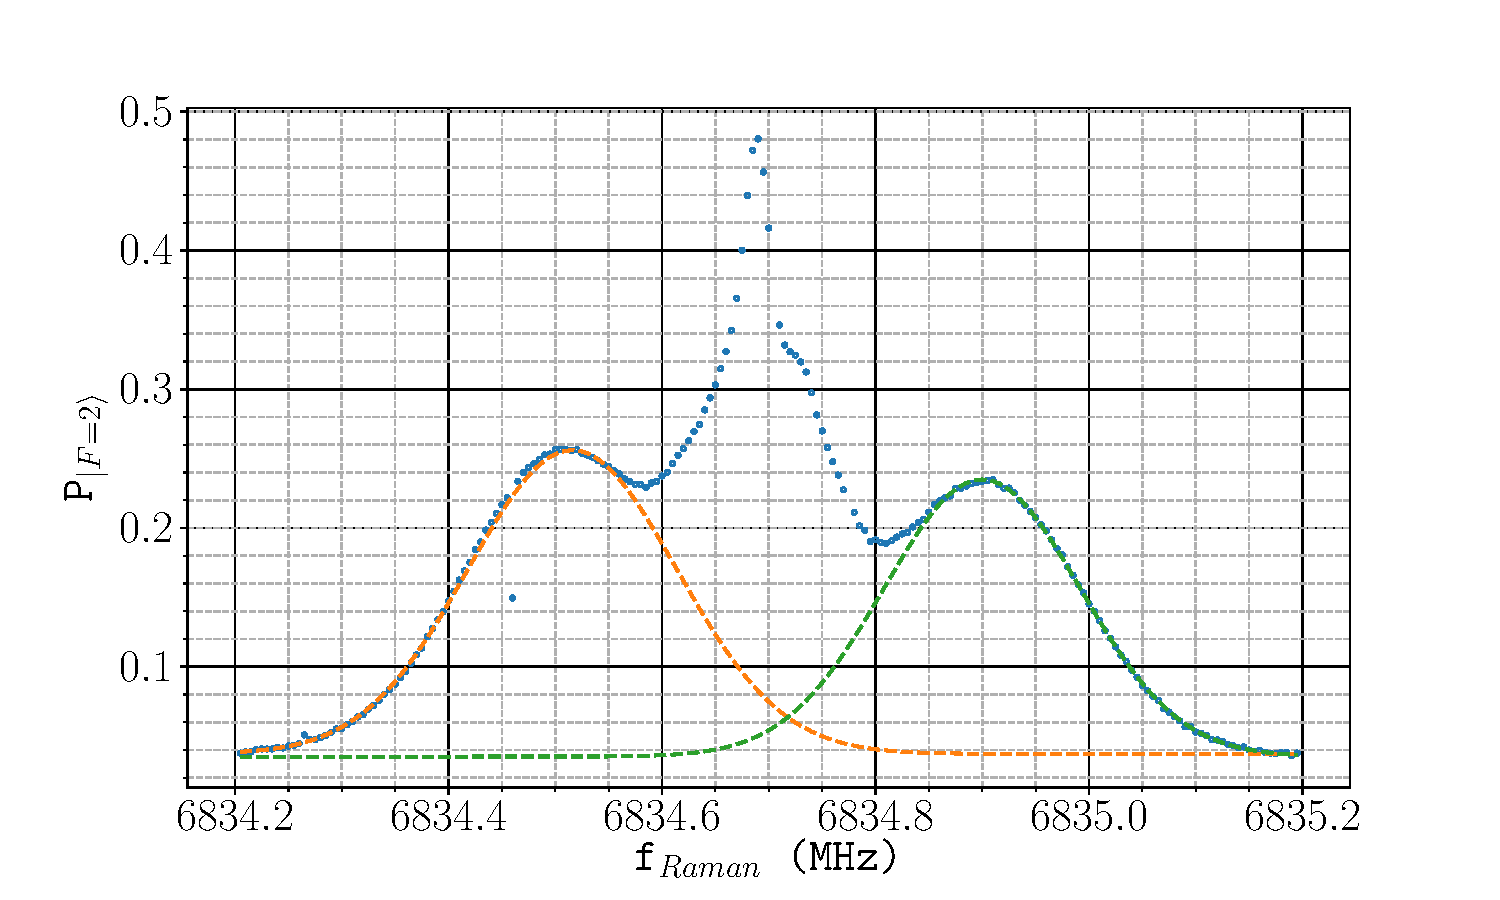
\includegraphics[width=0.7\textwidth]{raman_spectrum_inset}
  \caption[\(\Delta m = 0\) transition spectrum.]{Transition spectrum showing the \(\Delta m = 0\) transition
  from \(\ket{1,0}\). The orange and green dashed lines are fits to a
Doppler-broadened lineshape for each of the counter-propagating
profiles.}
  \label{fig:raman_spectrum_inset}
\end{figure}

\subsection{Cancelling the Differential ac Stark
Shift}\label{subsec:light_shift}
It is worth considering the effects of ac Stark shifts on the atom
interferometer~\cite{Gauguet2008}. They are intrinsically related to the
effective Rabi frequency and as such, cannot be avoided. Each light
beam couples each hyperfine ground state to intermediate states in the
5$P_{1/2}$ and 5$P_{3/2}$ levels in Rubidium-87. The total ac Stark
shift of each level\footnote{The ac Stark shift term
in~\EquationRef{eq:raman_ac_stark} was defined assuming that each
field $\textbf{E}_j$ couples to only one ground state $\ket{j}$. Here,
we do not make that assumption.} is a sum over the shift from each
coupled excited state
\begin{equation}
  \Omega_j^\text{ac} = \sum_{ik} -\frac{|\Omega_{ijk}|^2}{4\Delta_{ijk}}
\end{equation}
in terms of the one-photon Rabi frequencies \(\Omega_{ijk}\) and detunings \(\Delta_{ijk}\) where the index $i = 1,2$ labels each light field, $j = 1,2$ labels
each hyperfine ground state and $k$ labels each excited state that is
coupled by a dipole transition to $j$. From the free evolution of the atom's internal state, there is a contribution to the phase along each path that is
proportional to the sum of the light shifts of each hyperfine ground
state $(\Omega_1^\text{ac} +
\Omega_2^\text{ac})$. For an interferometer pulse separation of $T=
$\sivalue{25}{\ms}, the maximal separation of each path is
$\frac{\hbar k_\text{eff}}{m} T$ = \sivalue{300}{\micro\m}. Close to
the centre of the Raman beams, there is a negligible variation of
intensity over this distance, so the sum of the ac Stark shifts of
each state should not lead to an observable interferometer phase
shift.
\par\noindent
The Raman resonance depends on the difference in energy of the two
states $\hbar(\omega_2 - \omega_1)$. The ac Stark shifts of each state
therefore leads to a contribution to the detuning that depends on the differential ac Stark shift \(\delta^\text{ac}
= \Omega_2^\text{ac} - \Omega_1^\text{ac}\). can lead to an observable
phase shift. Using the results from Ref.~\cite{Weiss1994} for \(\pi\)
and \(\frac{\pi}{2}\) pulses, the phase shift to a Mach-Zender type
interferometer is
\begin{equation}
  \Delta \Phi^\text{ac} =
  \frac{\delta_3^\text{ac}}{\Omega_\text{eff}} - \frac{\delta_1^\text{ac}}{\Omega_\text{eff}} 
 \label{eq:diff_phase}
\end{equation}
where \(\delta_3^\text{ac}\) and \(\delta_1^\text{ac}\) are the ac
Stark shifts of the last and first \(\frac{\pi}{2}\) pulses,
respectively, and $\Omega_\textnormal{eff}$ is the effective Rabi
frequency defined in~\EquationRef{eq:rabi_raman_sum}. Note that there
is no sum over the beam index $k$, because in making the rotating wave
approximation, terms which contain $\Delta_{21k}$ and $\Delta_{12k}$
are dropped as they oscillate much faster than the retained terms. 
\par\noindent
As the atoms fall
under gravity, they move through the Raman beam profile and experience
the interferometer pulses at different intensities. To the extent that
there is a light shift of the clock transition, this can produce a
non-zero interferometer phase. Fortunately, it is possible
to eliminate such a shift using an appropriate choice
of intensity and detuning of the Raman lasers. This can be seen by
first writing out the differential ac Stark shift
\begin{equation}
  \delta^\text{ac} = \Omega_1^\text{ac} - \Omega_2^\text{ac} = \sum_{ik}
  \frac{\lvert\Omega_{i1k}\rvert^2}{4\Delta_{i1k}} - \sum_{ik}
  \frac{\lvert\Omega_{i2k}\rvert^2}{4\Delta_{i2k}} 
  \label{eq:diff_shift}
\end{equation}
When both Raman beams are red-detuned from
all the one-photon transitions, both terms
in~\EquationRef{eq:diff_shift} are strictly negative. Therefore,
\(\delta^\text{ac}\) can be cancelled by choosing the correct
intensities for each Raman beam. A plot of \(\delta^{\text{ac}}\)
for various Raman beam intensities as a function of the ratio between
the two Raman beams is shown in~\FigureRef{fig:light_shift_ratio}. There
is a ratio at which the differential ac Stark shift cancels and is
independent of the total intensity. The one-photon detuning $\Delta_R$
is defined such that the laser frequency $\omega_2^l$ is detuned from
the \trans{2}{3} transition (in the absence of light shifts) by
$\Delta_R$. The ratio that cancels
\(\delta^\text{ac}\) for increasing \(\Delta_R\) is shown
in~\FigureRef{fig:light_shift_detuning}. When \(\Delta_R\) is
\sivalue{1.13}{\giga\hertz} below the \trans{2}{3} transition, this
ratio is maximised. The differential ac Stark shift is cancelled when
the intensity ratio of light driving \(\ket{1,0}\) transitions to
\(\ket{2,0}\) transitions is \(\mathcal{R} = 0.583\). 
\begin{figure}[htbp!]
	\centering
	\def\svgwidth{\columnwidth}
	\subfloat[][]{\scalebox{0.45}{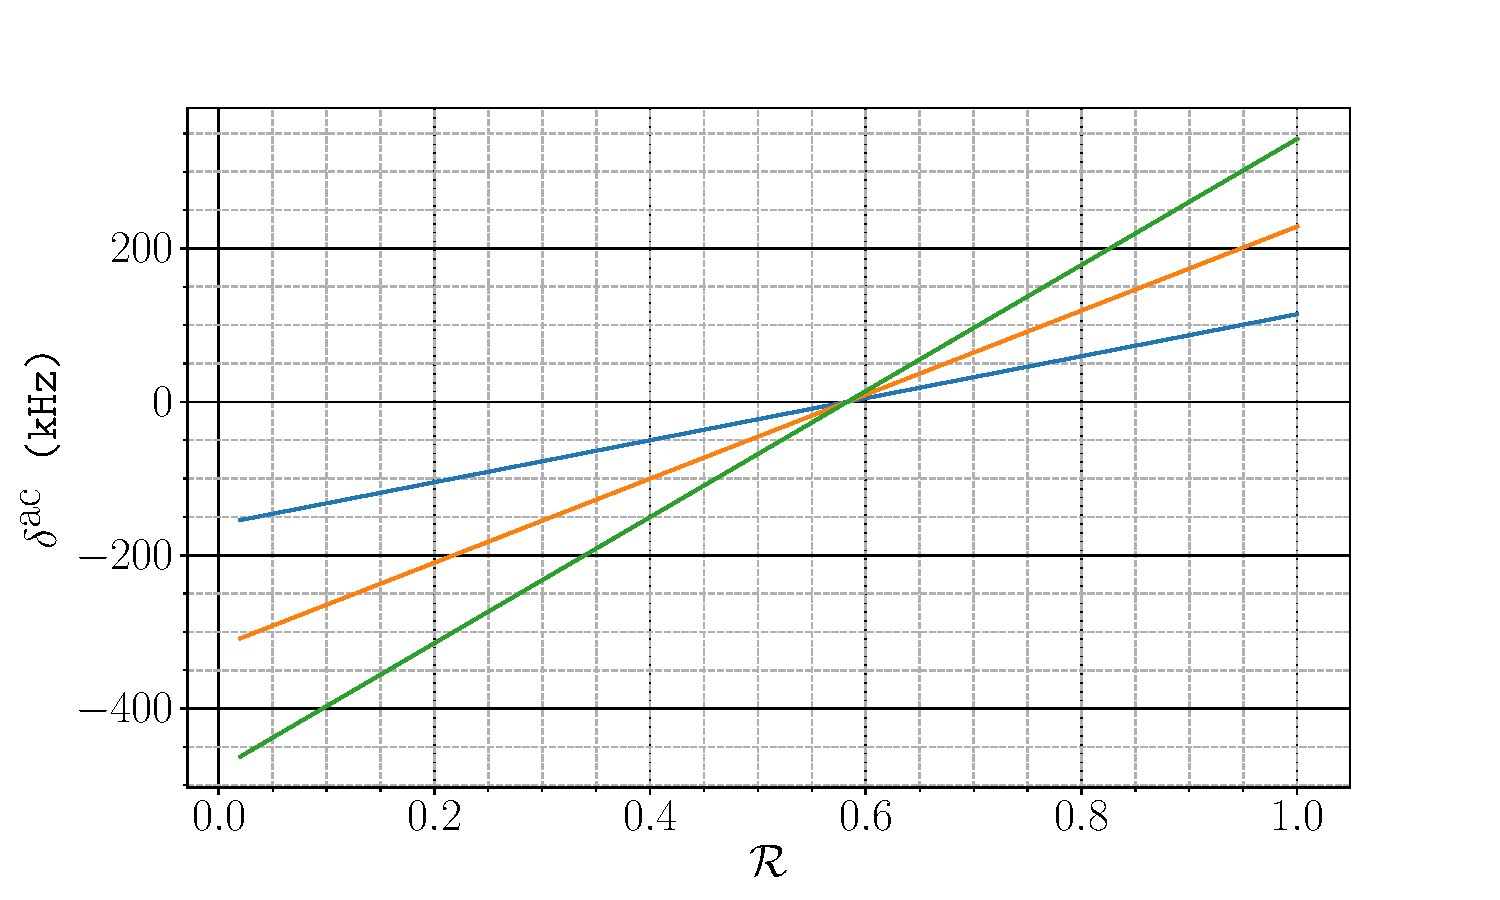
\includegraphics{light_shift_ratio}}\label{fig:light_shift_ratio}}\\
\subfloat[][]{\scalebox{0.45}{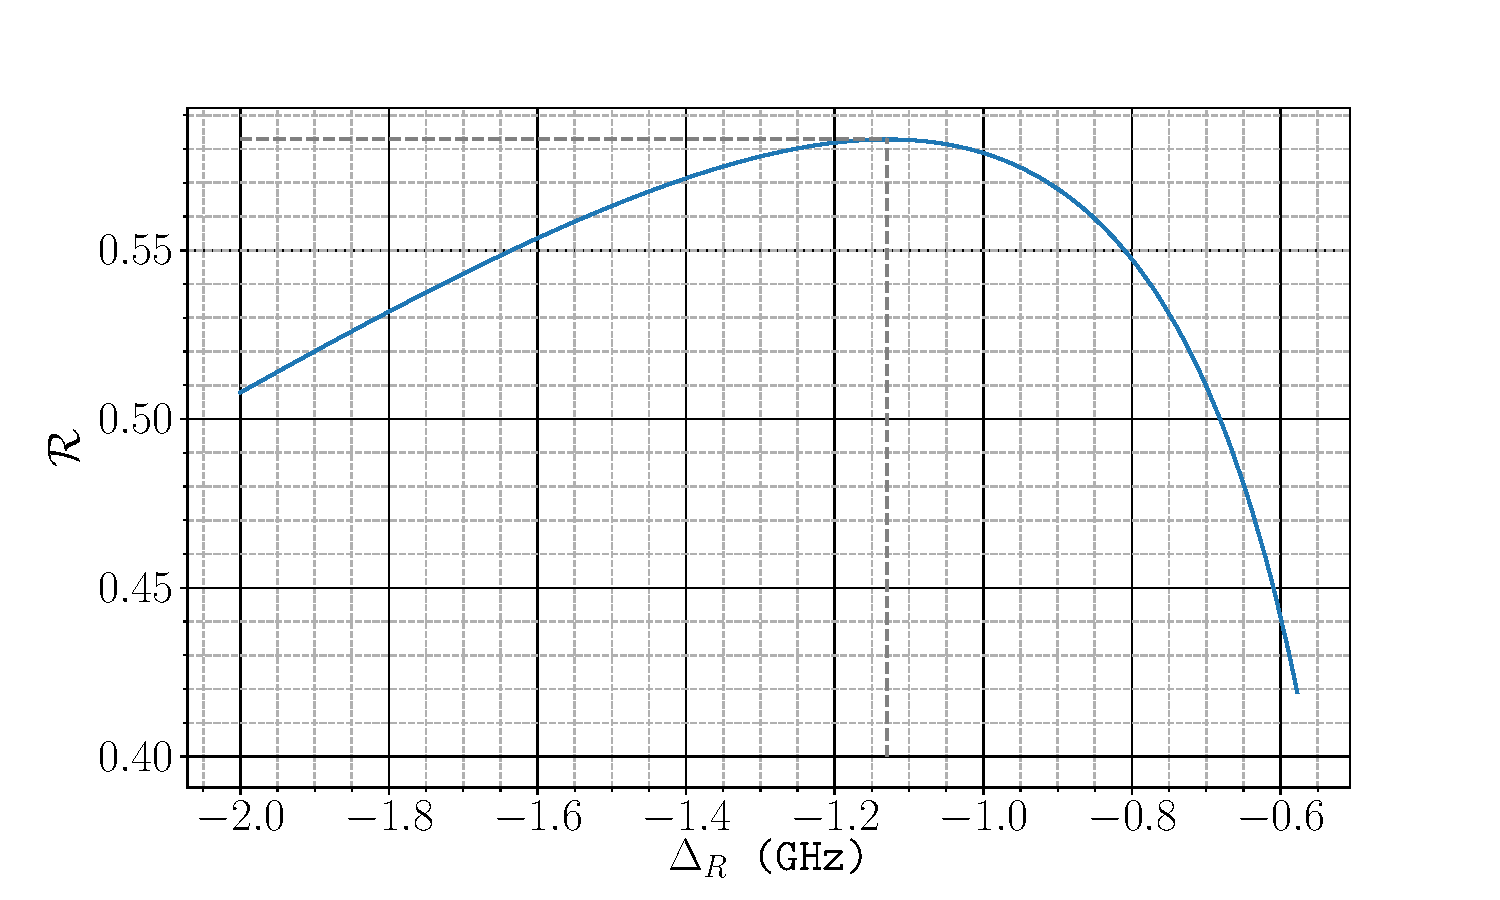
\includegraphics{light_shift_detuning}}\label{fig:light_shift_detuning}}\\
	\caption[Differential ac Stark shift as a function of two-photon
  detuning and Raman beam intensities.]{The effects of the Raman beam
  intensities and detuning on the differential ac Stark shift
  \(\delta^\text{ac}\).
\textbf{(a)} shows \(\delta^\text{ac}\) as a function of the intensity ratio
\(\mathcal{R}\) between the light which drives transitions from
\(\ket{1,0}\) to the light that couples to \(\ket{2,0}\) for the
two-photon detuning of \(\Delta_R = -\sivalue{1.13}{\giga\hertz}\)
used in the experiment. Example
intensities for the \(\ket{2,0}\) light are
\sivalue{100}{\watt\per\metre\squared} (blue),
\sivalue{200}{\watt\per\metre\squared} (orange) and
\sivalue{300}{\watt\per\metre\squared} (green). \textbf{(b)} shows how
the ratio for which \(\delta^\text{ac} = 0\) varies as \(\Delta_R\)
increases. The dashed lines indicate the value of \(\Delta_R\) used in
the experiment and its corresponding ratio of 0.583.}
	\label{fig:light_shift_plots}
\end{figure}
\par\noindent
It is not straight-forward to directly measure the intensity of
each Raman beam on the atoms, so the transition spectrum was used to cancel the
differential ac Stark shift and determine when the intensities of the
lasers are set to the appropriate
ratio. Experimentally, this was done by adjusting the power of the
pump lasers for the master and slave SolsTiS lasers. When the master
is seeded with \sivalue{10}{\watt} and the slave with
\sivalue{6.5}{\watt}, the differential ac Stark shift is eliminated.
\FigureRef{fig:cancelled_light_shift} shows the transition spectrum using two different effective Rabi
frequencies, corresponding to \(\pi\) pulse times of
\sivalue{22.5}{\micro\second} and
\sivalue{45}{\micro\second}. In this instance, the frequency difference of the two
co-propagating peaks, shown in blue and orange, is less than \sivalue{1}{\kilo\hertz}.
\begin{figure}[htpb!]
  \centering
  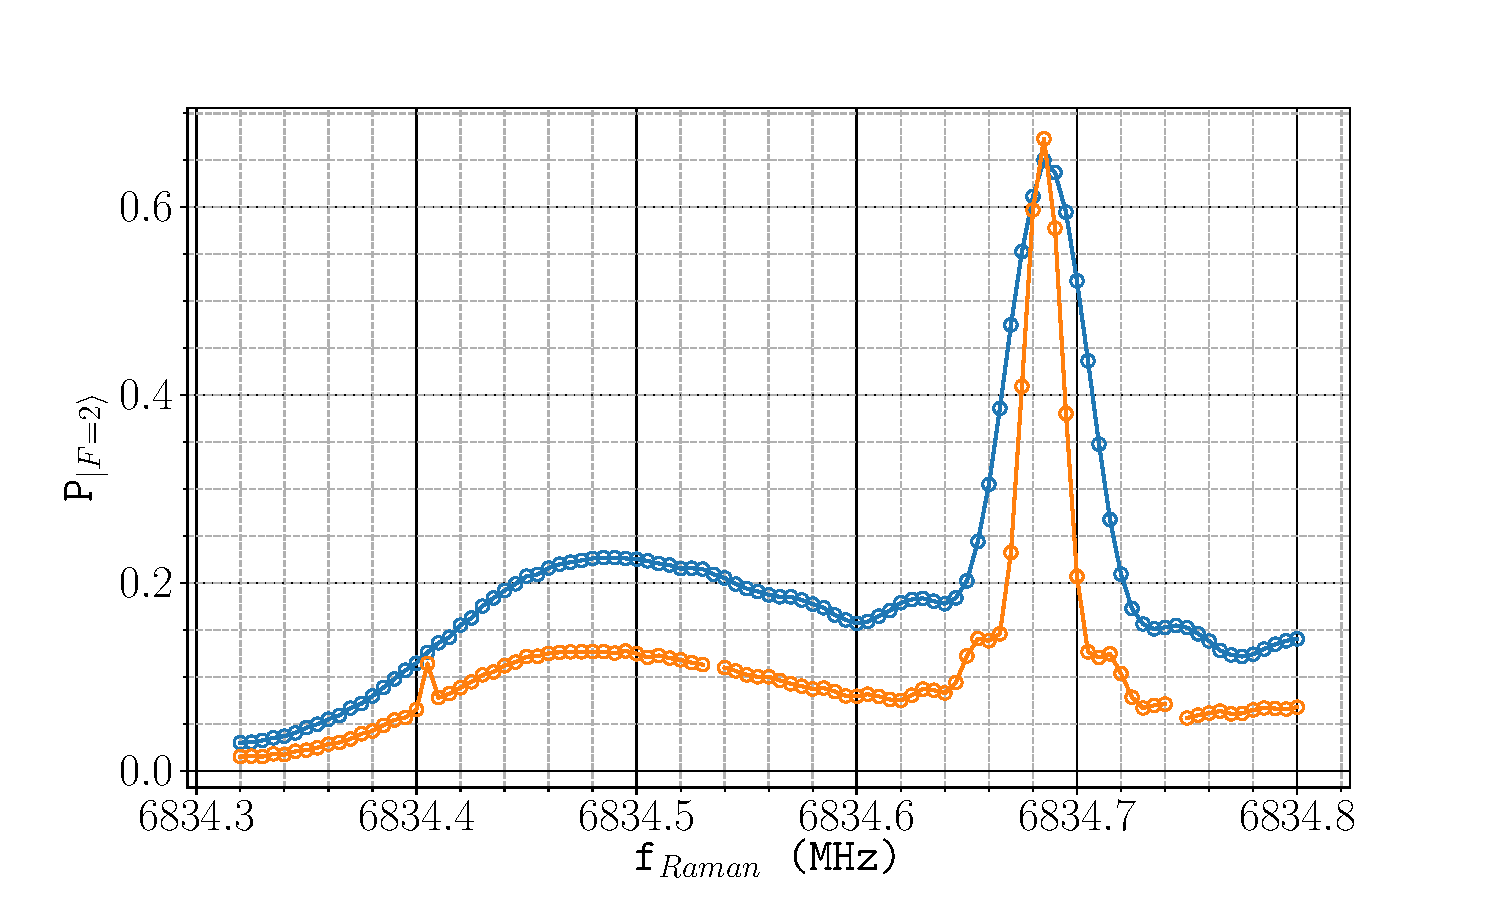
\includegraphics[width=0.7\textwidth]{cancelled_light_shift}
  \caption[Raman transition spectrum after cancelling the differential
  ac Stark shift.]{Raman transition spectrum after cancelling the differential
    ac Stark shift. The blue curve shows a pulse with a \(\pi\) pulse
  time of \sivalue{22.5}{\micro\second} and the orange shows the
  spectrum using a less intense pulse with a $\pi$-pulse time of
\sivalue{45}{\micro\second}.}
  \label{fig:cancelled_light_shift}
\end{figure}
There is also a shift of \sivalue{1.4}{\mega\hertz} from
\(f_\text{hfs}\).
This is a result of a
second-order Zeeman shift and corresponds to a field strength of
\sivalue{1.56}{\gauss}.
\subsection{Velocity-Selective Pulse}\label{subsec:vel_select}
The accelerometer has to use the velocity-sensitive transitions
induced by counter-propagating beams in order to be sensitive to
acceleration. In order for all the atoms to experience the same
desired pulse areas of $\pi/2-\pi-\pi/2$, it is necessary for the
Doppler width to be much less than the natural width arising from the
duration of the Raman pulses. In this apparatus, the laser cooling
gives a temperature of \sivalue{6}{\micro\kelvin}, for which the Doppler
width (FWHM) is \(\sigma_f = \frac{4 \sqrt{2 \ln(2)}}{\lambda}\sqrt{\frac{k_b T}{m}}
\approx\) \sivalue{140}{\kilo\hertz}. 
A $\pi$-pulse duration of \sivalue{6}{\micro\second} gives a
linewidth close
to this Doppler width, but the intensities required for this are above
what is attainable with our Raman laser. 
\par\noindent
We therefore reduce the Doppler width of the participating atoms
by first applying a long Raman pulse to select a subset of the population
with a narrower velocity spread~\cite{Moler1992}. This
velocity-selective pulse gives a narrower Doppler linewidth than the
subsequent shorter
interferometer pulses thereby ensuring that the Rabi frequencies are
reasonably homogeneous across the cloud of selected atoms.
\par\noindent 
Starting with a velocity distribution of atoms
described by a 1-D Maxwell-Boltzmann distribution all occupying the
\(\ket{1,0}\) state, the
population in \(\ket{2,0}\) after applying a Raman pulse is
distributed according to
\begin{equation}
  \text{P}_{\ket{2,0}}(v) = \frac{\Omega_\textnormal{eff}^2}{\Omega_\textnormal{eff}^2 + \delta^2}
  \sin\left(\sqrt{\Omega_\textnormal{eff}^2+\delta^2}\;\tau\right)^2 p(v)
  \label{eq:vel_selected_dist}
\end{equation}
where \(\delta\) is the Raman detuning defined
in~\EquationRef{eq:raman_detuning}, \(p(v) = \sqrt{\frac{m}{2\pi
k_B T}} e^{-\frac{m v^2}{2 k_B T}}\) is the velocity distribution and
\(\Omega_\textnormal{eff}\) is the effective Rabi frequency defined
in~\EquationRef{eq:rabi_raman_sum}. \FigureRef{fig:vel_selected_dist}
shows the expected
distribution of Doppler shifts in the selected atoms after a
\sivalue{6}{\micro\K} cloud has been driven by a $\pi$ pulse with a duration of
\sivalue{40}{\micro\second}.
The population that is stimulated
has a mean velocity shifted by twice the recoil velocity. In this
instance, the rms
Doppler shift is \(\sigma_f
=\)\sivalue{19.7}{\kilo\hertz}.
\begin{figure}[htpb!]
  \centering
  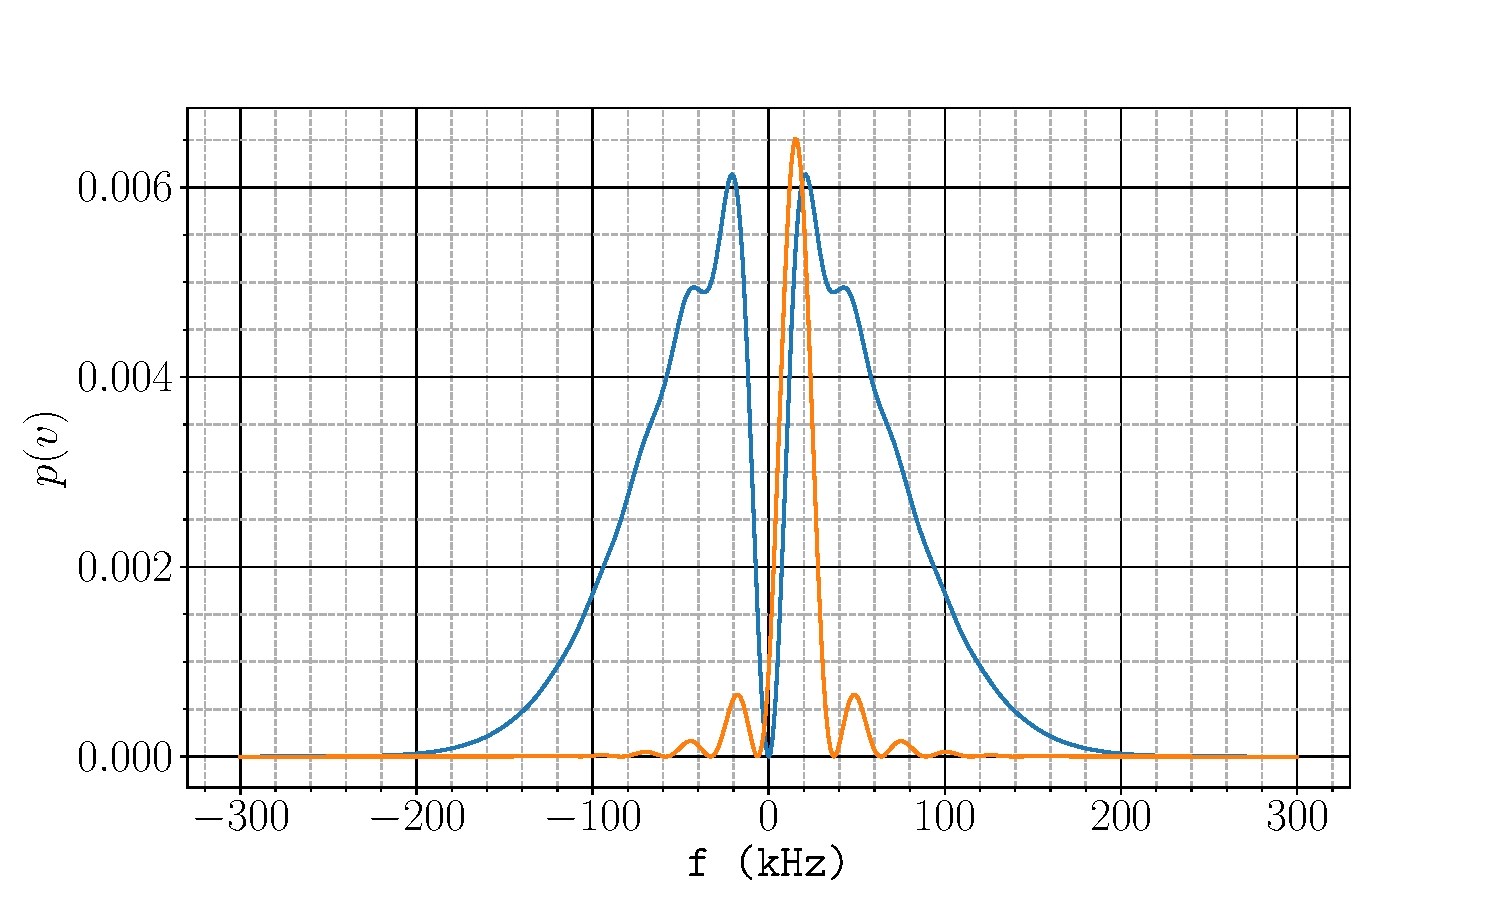
\includegraphics[width=0.7\textwidth]{vel_selected_dist.pdf}
  \caption[Simulated velocity distribution after a Raman $\pi$
  pulse.]{Calculated distribution of frequency shifts in the ensemble
    selected from a \sivalue{6}{\micro\kelvin}
  cloud by a \sivalue{40}{\micro\second} Raman \(\pi\)
pulse. Blue curve: atoms not selected. Orange curve: atoms selected.
Note the recoil shift of the selected atoms in addition to their
Doppler shifts. }
  \label{fig:vel_selected_dist}
\end{figure}
\subsubsection{Velocity-Selected Distribution}
The velocity distribution of atoms after the velocity selective pulse
can be measured using a second Raman pulse as a probe. This probe must
be much longer duration than
the velocity-selection pulse so that it gives even narrower
resonances. 
\FigureRef{fig:vel_select_chirp} shows a measurement of the transition
spectrum close to the peak of the Doppler-sensitive transition that is
greater in frequency than the Doppler-insensitive peak. The orange
curve shows the spectrum obtained before velocity selection, using a single Raman $pi$ pulse of
duration \sivalue{40}{\micro\s}. The blue curve, which illustrates the
distribution of atoms after velocity selection, is obtained by first
applying a
\sivalue{40}{\micro\second} \(\pi\) pulse with a Raman beat frequency
\(f_v = \) \sivalue{6834.51}{\mega\hertz}. This prepares atoms in
\(\ket{1,0}\), then the atoms which remain in
\(\ket{F=2}\) are blown away. After \sivalue{10}{\milli\second}, a
\sivalue{80}{\micro\second} \(\pi\) pulse transfers some of the
remaining population back into \(\ket{2,0}\). The frequency of the
probe pulse is varied by chirping the Raman laser beat frequency. In
this instance, the power of the \sivalue{80}{\micro\s} pulse was not tuned to give a \(\pi\)
pulse area so the measured population is not indicative of the maximum
driven by the Raman transition. The red curve shows a fit to a
Doppler-broadened lineshape, which gives an effective temperature
of around \sivalue{1}{\micro\K}. Comparing this to the peak from
before velocity selection, it is clear that the velocity
distribution of the selected atoms is much narrower. 
\begin{figure}[htpb!]
  \centering
  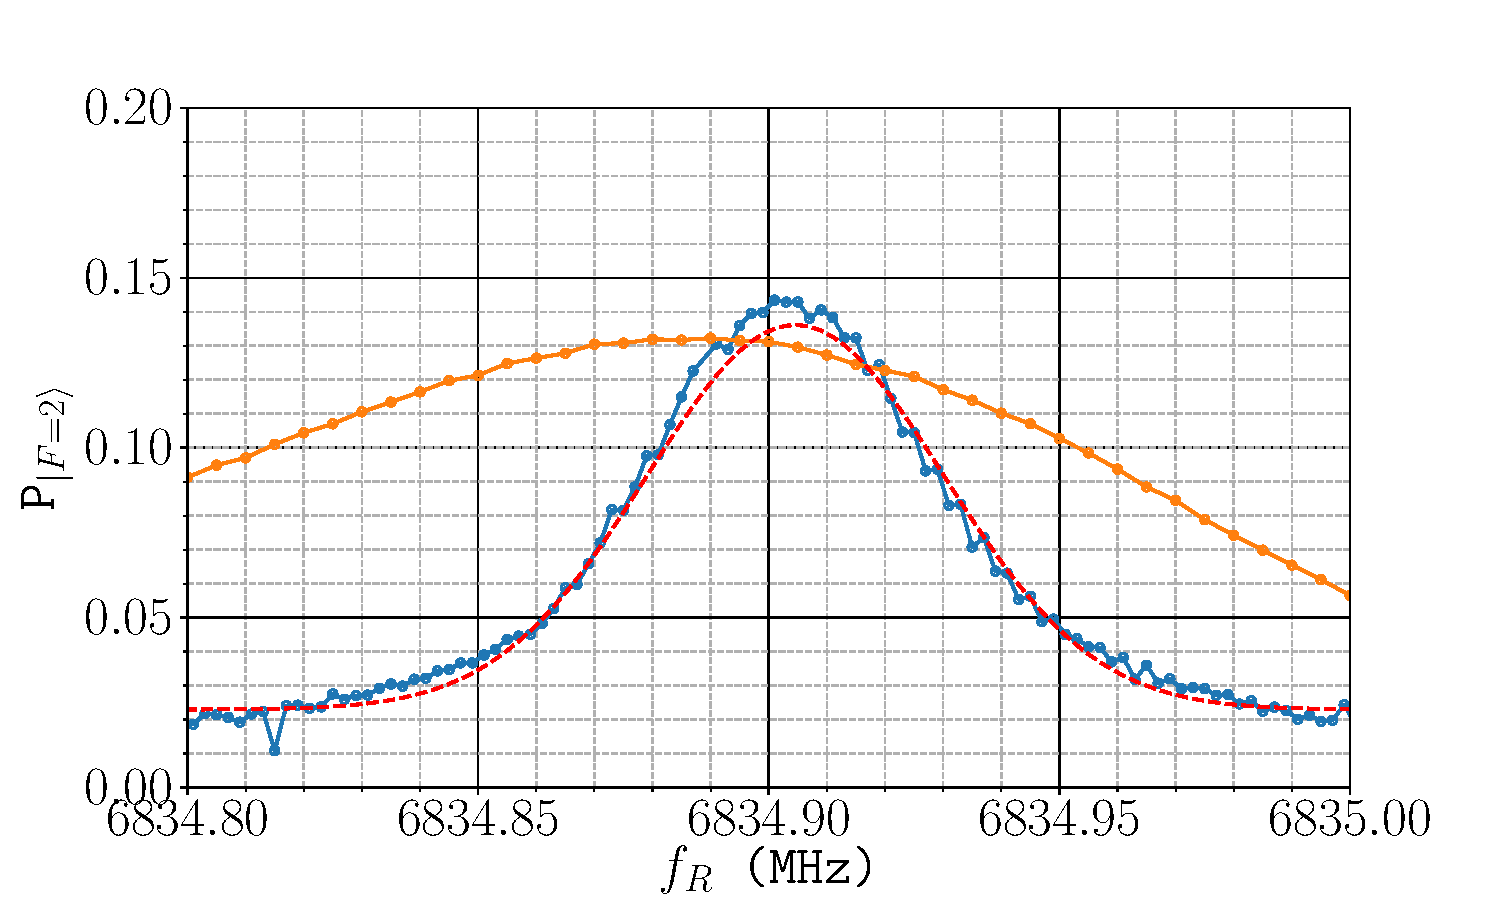
\includegraphics[width=0.7\textwidth]{RamanChirp.pdf}
  \caption[$\ket{F=2}$ population after a velocity-selective Raman
  $\pi$ pulse.]{\(\ket{F=2}\) population after a Raman pulse at a frequency
    \(f_v =\)\sivalue{6834.51}{\mega\hertz} transfers atoms to
    \(\ket{1,0}\). This distribution is probed by
  applying a narrow pulse at a frequency \(f_{R}\). The population
measured in \(\ket{F=2}\) is shown in blue. The red dashed line is a
fit to the Doppler-broadened
transition peak. The orange curve shows
transition spectrum (without velocity selection) from a $pi$-pulse
of duration \(\tau = \)\sivalue{40}{\micro\s}.}
  \label{fig:vel_select_chirp}
\end{figure}
\subsection{Interferometer Pulses}\label{subsec:int_pulses}
The power settings needed to make Raman $\pi$ and $\pi/2$ pulses were
empirically determined by observing Rabi oscillations. These are shown
in~\FigureRef{fig:rabi_oscillation}. For a $\pi$ pulse, the Raman
laser power was
set so that the Rabi oscillation reached its maximum after a pulse duration of
\(\tau = \)\sivalue{15}{\micro\s}. It is clear that the oscillations
are rapidly damped. This dephasing rate depends on the
time at which the pulse is applied. Since the atoms are at different
positions in the beam, this suggests that the dephasing is caused by a
spatial variation of the Rabi frequency. This is largely a result of
irregularities in the Raman beam intensity profile from defects in
the two small aspheric lenses. The Gaussian intensity distribution of each beam
is unlikely to cause such a fast dephasing, since the atoms remain
close to the centre of the beam. At longer pulse durations,
spontaneous decay from the intermediate states of the Raman transition
becomes apparent.
\begin{figure}[htpb]
  \centering
  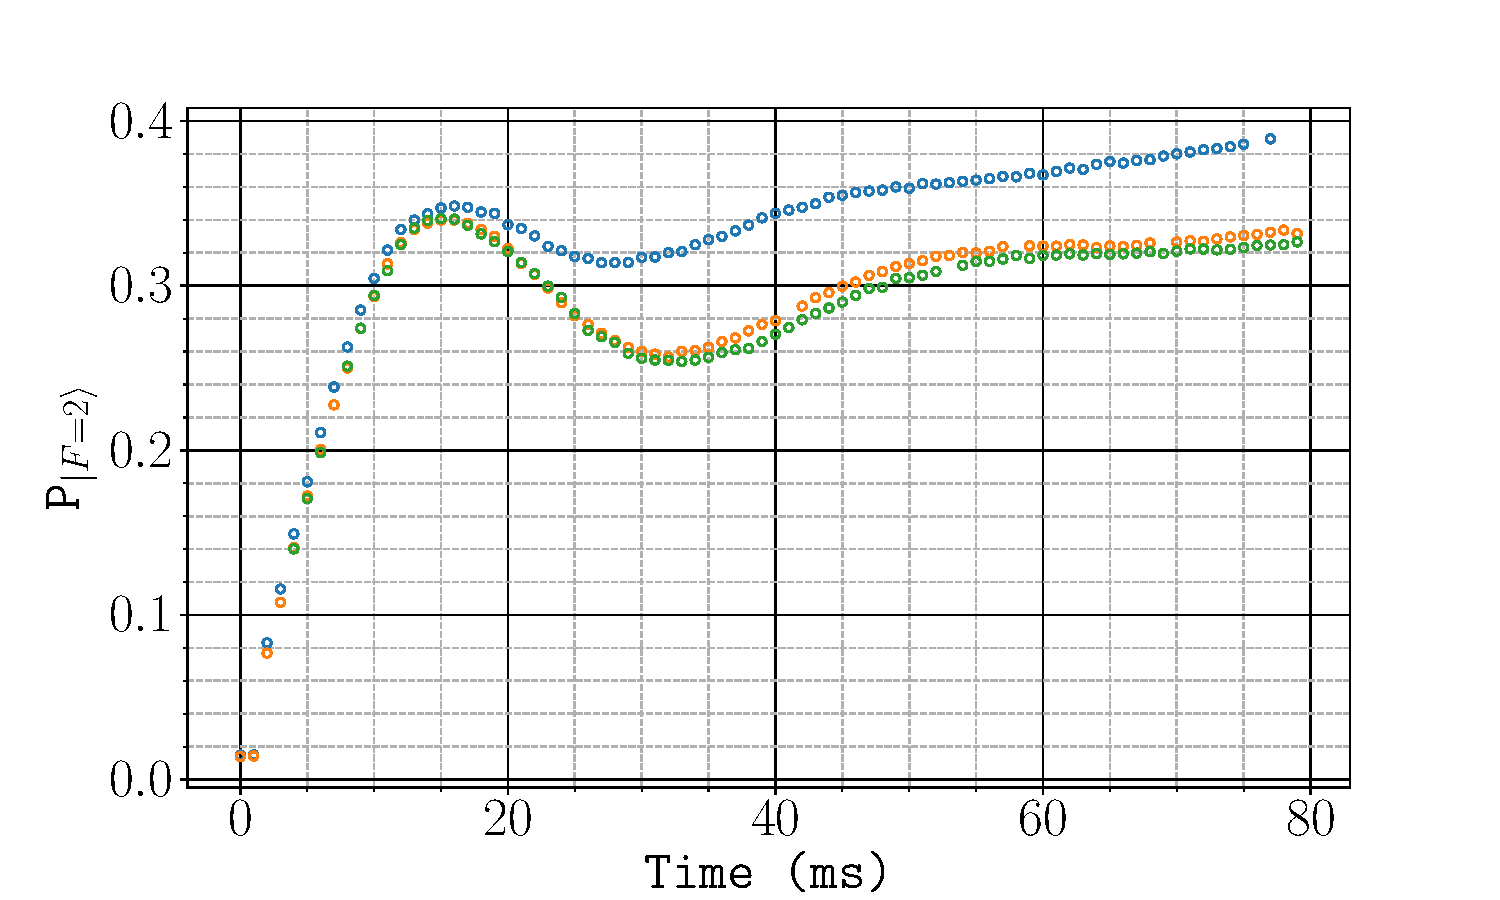
\includegraphics[width=0.8\linewidth]{SinglePulses.pdf}
  \caption[Rabi oscillations between the $\ket{1,0}$ and $\ket{2,0}$
    states.]{Rabi oscillations between the $\ket{1,0}$ and $\ket{2,0}$
    states. Each pulse occurs at different times after the \ac{mot} is
    released. The times shown are \sivalue{13}{\ms} (blue),
  \sivalue{23}{\ms} (orange) and \sivalue{33}{\ms} (green). Full
  population transfer is not observed due to the atoms in $\ket{1,\pm
1}$ which have not been removed. }
\label{fig:rabi_oscillation}
\end{figure}
\section{Noise}\label{sec:atomint_sensitivity}
This section presents a discussion of the identified sources of
noise in the interferometer and their effects on the sensitivity to
accelerations. It begins with a discussion of the noise that arises
from detecting atoms in~\SectionRef{subsec:detection_noise}. This
defines an uncertainty in measuring the occupation probability, which then used to
express the corresponding acceleration uncertainty
in~\SectionRef{subsec:accel_uncert}. The Allan variance used to characterise
the stability of the interferometer signal is defined
in~\SectionRef{subsec:allan_variance}. The sensitivity function and an analytic method
for calculating the influence of random phase fluctuations is given
in~\SectionRef{subsec:sens_func}. This is applied to phase noise from
the Raman laser in \SectionRef{subsec:laser_phase} and external
vibrations in~\SectionRef{subsec:vibration_noise}. Finally, the
section concludes with a summary of the identified sources of noise
in~\SectionRef{subsec:noise_sources}.
\subsection{Detection Noise}\label{subsec:detection_noise}

Each measurement of the number of atoms has an uncertainty due to
random processes that influence the voltage measured by the detector. These errors
combine to give an uncertainty in the interferometer phase and
hence, acceleration. It is worth distinguishing between the different
sources of noise in measuring the occupation probability
$\text{P}_{\ket{F=2}}$. Fluctuations in the number of atoms and detected
photons lead to an uncertainty in the measured voltages that
correspond to $N_2$ and $N_\text{Tot}$. It is essential that the
photo-detector used is sensitive enough to ensure that this does not
limit the sensitivity~\cite{Rocco2014}. A more fundamental limitation
is the noise that arises when an atom is projected into either the
$\ket{1,0}$ state or the $\ket{2,0}$ state. In what follows, these
three sources of detection noise are discussed in the context of the
detection sequence previously described
in~\SectionRef{subsec:detection_sequence}. 
\subsubsection{Atom and Photon Number Fluctuations}
The random processes by which atoms are loaded and cooled in the
initial stages of the experiment, as well as the random direction a
photon is spontaneously emitted mean that both the total number of
atoms after interferometry and the number of photons arriving at the
detector within a given time duration will have shot noise
fluctuations. The voltage measured by the detector, as defined
in~\EquationRef{eq:pd_signal}, is proportional to the number of atoms
scattering the incident light. Therefore, the variance in the measured
voltage due to atom and photon shot noise fluctuations are 
\begin{align}
  \sigma_\text{at,v}^2 &= \alpha^2 \eta^2 R_\text{sc}^2 n_\text{at}\\
  \sigma_\text{p,v}^2 &= \alpha^2 \eta R_\text{sc} n_\text{at} 
  \label{eq:atom_photon_noise}
\end{align}
where $\alpha = \hbar \omega G$ and the subscripts ``at'' and ``p'' refer to atoms and photons,
respectively. Of the two, \(\sigma_\text{at,v}\) dominates provided at least one photon
per atom is detected. As previously discussed
in~\SectionRef{subsec:photodiode_setup}, around 7 photons per atom
are detected, so this is certainly the case. For the detection parameters previously defined, the shot noise is equal to around \sivalue{46.5}{\nano\volt} per atom. 
The standard deviation of the detected voltage during background light
measurements was on the order of \sivalue{80}{\micro\volt}. Since at
least \num{1e6} atoms are detected, the noise from background light
fluctuations is negligible.  

\subsubsection{Quantum Projection Noise}
The occupation probability $\text{P}_{\ket{F=2}}$ is determined by measuring the ratio
$\frac{N_2}{N_\text{Tot}}$. In
measuring both the number of atoms in $\ket{F=2}$ and the total number of atoms, the contribution of atom shot
noise to an uncertainty in $\text{P}_{\ket{F=2}}$ is suppressed. However, for a
fixed number of atoms there is still an uncertainty due to the
projection of an atom's internal state onto the $\ket{1,0}$ and
$\ket{2,0}$ states. This is the standard quantum limit -- the minimum
uncertainty that can be reached for an ensemble of atoms prepared in
the same internal state~\cite{Bollinger1996}. 
To derive the uncertainty in $\text{P}_{\ket{F=2}}$, we first make the assumption
that there are atoms in $m_F=\pm 1$, as
in~\SectionRef{subsec:atom_number_bias}, which are detected but do not
contribute to the interferometer. The total number of atoms is
$N_\text{Tot}$. Similarly, $n_2$ atoms detected in $\ket{F=2}$, which
has an average value denoted as $\langle N_2 \rangle$ and a mean
occupation probability $\langle p_2 \rangle$. If $n_{10}$ is the
number atoms prepared in $\ket{1,0}$, it follows that the mean and
variance of $n_2$ are given by
\begin{align}
  \langle N_2 \rangle &= \langle p_2 \rangle \\
  \Delta N_2 &= n_{10} \Delta p_2 = n_{10} \langle p_2 \rangle \langle
  p_1 \rangle \label{eq:proj_noise}
\end{align}
where $\langle p_1 \rangle$ is the average occupation probability of
$\ket{F=1}$ after interferometry. The measured probability is given by
\begin{align}
  \text{P}_{\ket{F=2}} &= \frac{\langle p_2 \rangle n_{10} \pm \sqrt{n_{10}
  \langle p_2 \rangle \langle p_1 \rangle}}{n_{10}(1+\epsilon)}
  \nonumber \\
                &= \frac{\langle p_2 \rangle}{1+\epsilon} \pm
                \frac{1}{1+\epsilon} \sqrt{\frac{\langle p_2 \rangle
                \langle p_1 \rangle}{n_{10}}} 
                \label{eq:prob_noise}
\end{align}
where as before $\epsilon$ is the ratio of the number of atoms in $m_F = \pm 1$ to
the number in the interferometer and it is assumed that this ratio
does not fluctuate. Without any inhomogeneity in the
Rabi frequency\footnote{Atoms which experience different pulse areas
  have different phase shifts. The interferometer signal is a
convolution of these. In which case, the contribution to the detection
noise from the projection noise of each atom is less straight-forward.
For simplicity, it is assumed here that the only loss
in fringe contrast is due to background atoms.}, the average occupation probabilities are 
$\langle p_2 \rangle = \sin^2(\Delta \Phi/2)$ and $ \langle p_1
\rangle = \cos^2(\Delta \Phi/2)$. In terms of the interferometer phase
difference $\Delta \Phi$, \EquationRef{eq:prob_noise} becomes
\begin{equation}
  \text{P}_{\ket{F=2}} = \frac{1-\cos(\Delta \Phi)}{2(1+\epsilon)} \pm
  \frac{1}{2(1+\epsilon)}\frac{\sin(\Delta \Phi)}{\sqrt{n_{10}}}
\end{equation}
A useful measure of the interferometer's sensitivity is given by the
ratio of the noise to the fringe amplitude which is
\begin{equation}
  S = \frac{\sin(\Delta\Phi)}{\sqrt{n_{10}}}
  \label{eq:sens_proj}
\end{equation}
and is independent of $\epsilon$. At the mid-point
of a fringe $\Delta \Phi = \frac{\pi}{2}$, this is maximised and the
interferometer is most sensitive to changes in $\Delta \Phi$. A
relation between the uncertainty in $\text{P}_{\ket{F=2}}$ and the
interferometer phase is derived in~\SectionRef{subsec:accel_uncert}.

\subsubsection{Photodiode Technical Noise}
In order for the detection noise
be dominated by the quantum projection noise, the detector must be sensitive
enough that it has a \ac{nep} much lower than the noise in the optical
power detected. The \ac{nep} of a detector is defined as the
equivalent optical power which gives a signal-to-noise ratio of 1
after an integration time of \sivalue{0.5}{\second}. The photodiode
signal is amplified so it is convenient
to express the technical noise as a voltage density, by multiplying it by the
amplifier gain. Hence, the
voltage density of a detector whose sensitivity is equivalent to the
voltage corresponding to the quantum projection noise for an
integration time \(\tau_D\) is given by
\begin{equation}
  V^2_\text{at} =
  \frac{1}{2\tau_D}\eta \hbar \omega G R_\text{sc}\Delta N_\text{proj}
  \label{eq:nep}
\end{equation}
where $\Delta N_\text{proj} = \sqrt{N_\text{proj}}$ is the variance in
the number of atoms detected due to the projection of atoms onto the
states $\ket{1,0}$ and $\ket{2,0}$. If the signal is detected for $\tau_D =$ \sivalue{200}{\micro\s},
multiplicative factor that relates $V_\text{at}$ to
$\Delta N_\text{proj}$ is \sivalue{6.7e-12}{\volt\squared\per\hertz}.
\par\noindent
Technical noise in the detector typically arises from multiple electronic processes -- such as Johnson noise and shot noise in
the current~\cite{Howard2002}. The technical noise of the detector can
be estimated by measuring the output voltage when no light is
collected. A plot of the power spectral density of the photodiode is
shown in~\FigureRef{fig:noise_source_psd} taken
with a sampling frequency of \sivalue{200}{\kilo\hertz}. The
photodiode was covered and the output voltage was sampled for
\sivalue{2}{\second}. The power spectral density has been calculated
using Welch's method~\cite{Welch1967}. The data are partitioned before
calculating the Fourier transform of each subset and taking the
average. This has the effect of reducing the variance in the estimated
power spectrum at the expense of reducing the frequency resolution.
Below \sivalue{10}{\kilo\hertz} the power spectral density is close
to uniform with a value of around
\sivalue{5e-13}{\volt\squared\per\hertz}, which corresponds to a
noise-equivalent power of \sivalue{391}{\femto\W\per\hertz\tothe{1/2}}.
For higher frequencies, the power spectral density starts to
increase. The plot also indicates the corresponding voltage noise
density to reach the
quantum projection noise limit after detecting for a duration $\tau =
2/f$ for atom numbers of 
of n\(_{10} =\) \num{5e6} and \num{1e6} with the previously
defined output voltage per atom of $\sivalue{30}{\nano\volt}$. The
dot-dashed line corresponds to a detection time of
$\sivalue{200}{\micro\s}$. At this duration, the detection noise is
limited by the technical noise in the detector. This issue certainly
needs to be addressed to ensure that the detection noise reaches the
fundamental projection noise limit. 
\begin{figure}[htpb!]
  \centering
  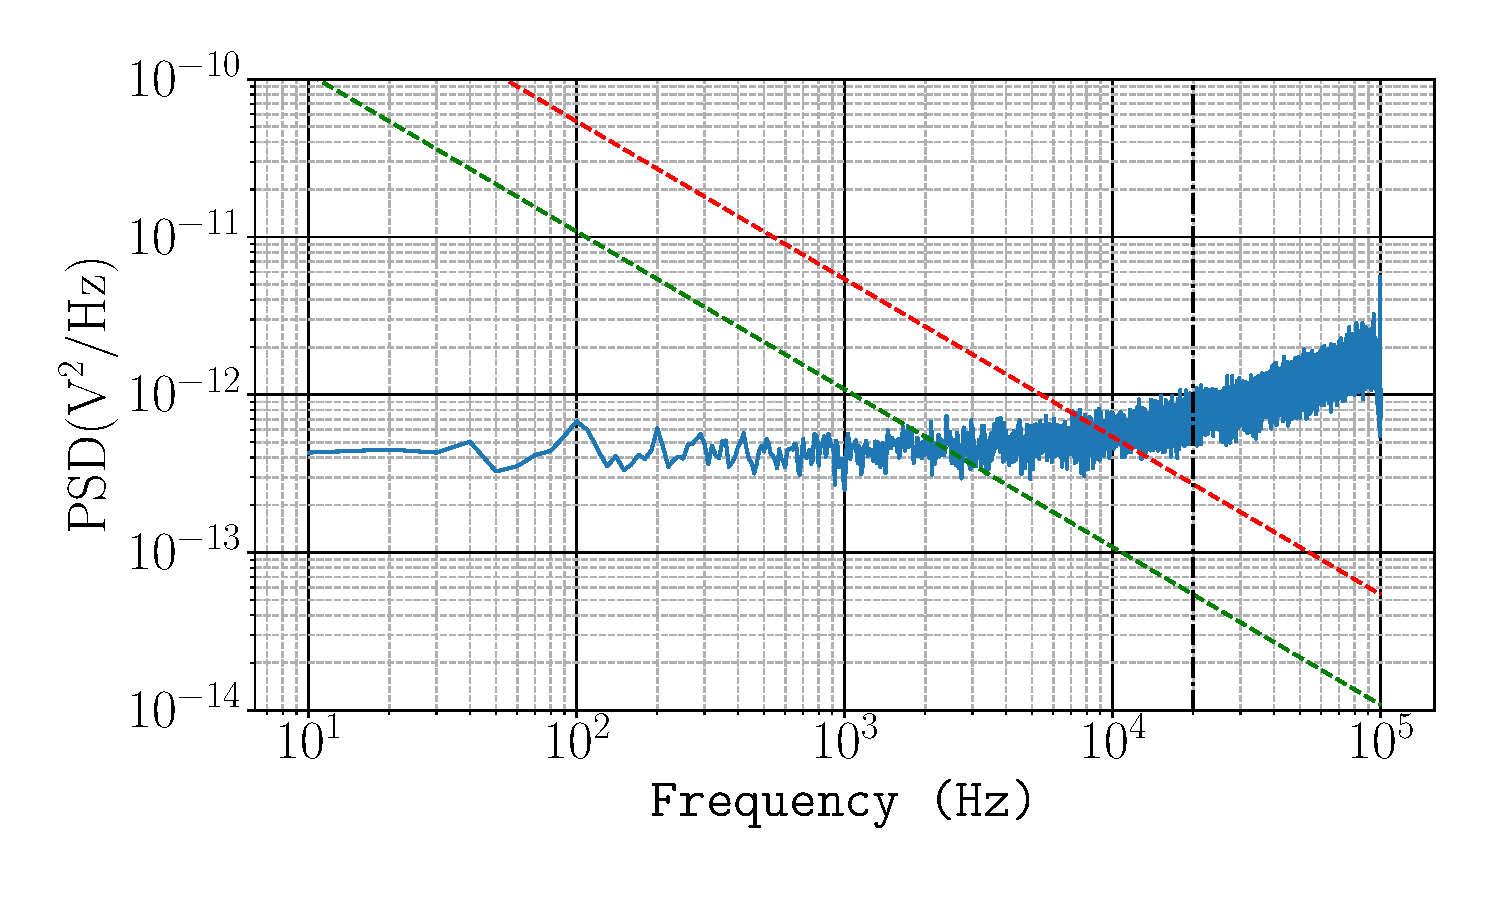
\includegraphics[width=0.7\textwidth]{noise_source_psd}
  \caption[Photodiode power spectral density]{Power spectral density
    of the voltage from the amplified photodiode signal
  sampled for \sivalue{2}{\second} at a rate of
\sivalue{200}{\kilo\hertz}. The red and green dashed lines indicate
the required voltage noise density to equal the quantum projection
noise level
after integrating for \(\tau = 2/f\)\sivalue{}{\s} for atom numbers of
\num{5e6} and \num{1e6}, respectively. The dot-dashed line indicates
the frequency corresponding to a detection time of
\sivalue{200}{\micro\s}.}
  \label{fig:noise_source_psd}
\end{figure}
%\par\noindent
%Averaging the detection signal over a time \(\tau\) has the effect of
%filtering the signal above the Nyquist frequency \(f_n = 1/(2 \tau)\).
%The variance in the averaged voltage over successive shots
%i.e. the Allan variance, is related to the power spectral density as
%follows
%\begin{equation}
%  \sigma^2_\text{av}(\tau) = 2 \int_0^\infty \frac{\sin(\pi \tau f)^4}{(\pi \tau f)^2}S(f)\;\mathrm{d}\;f
%  \label{eq:av_psd}
%\end{equation}
%Using~\EquationRef{eq:av_psd}, it is possible to determine the
%detection time required to reduce the shot-to-shot variance below the
%quantum projection noise level. \FigureRef{fig:detecion_av} shows the Allan deviation for increasing
%integration time. Above it shows the $\tau^{-1/2}$ dependence
%characteristic of uncorrelated white noise. The red and greed curves
%show the voltages corresponding to the quantum projection noise
%for the same numbers of atoms used
%in~\FigureRef{fig:noise_source_psd}. At the integration time of
%\sivalue{200}{\micro\second}, the detector noise
%is close to \sivalue{5}{\micro\volt} -- well below the quantum
%projection noise level.
%\begin{figure}[htpb!]
%  \centering
%  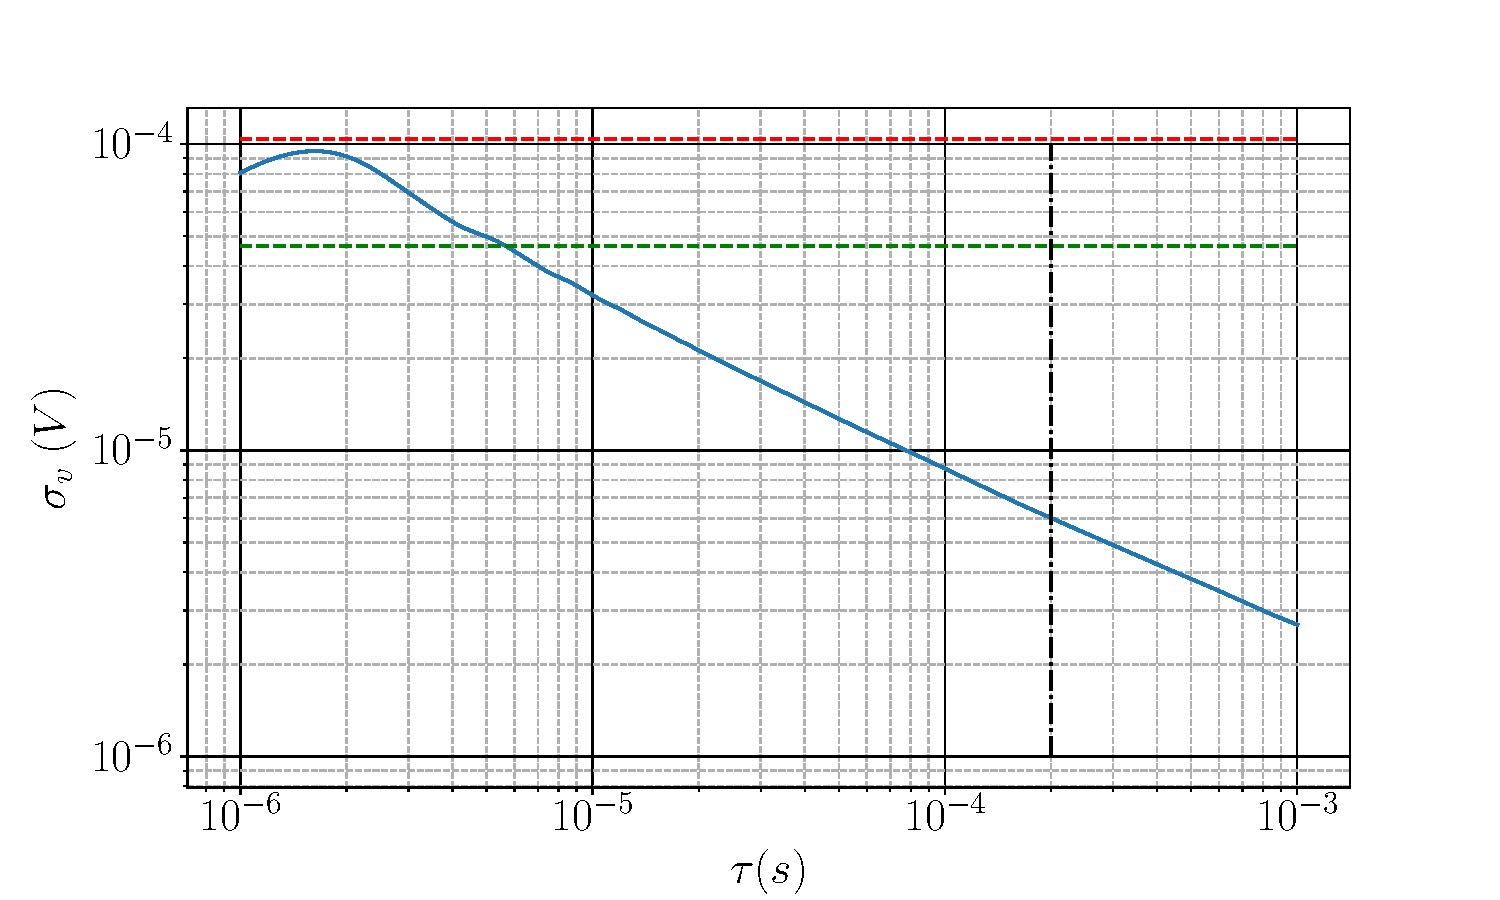
\includegraphics[width=0.7\textwidth]{detection_av}
%  \caption[Allan deviation of Photodiode voltage.]{Allan deviation of
%    the amplified photodiode voltages for increasing
%  integration time \(\tau\). The red and green dashed lines are the
%quantum projection noise levels for the atom numbers used
%in~\FigureRef{fig:noise_source_psd}. The black dot-dashed line indicates the
%integration time of \sivalue{200}{\micro\second} used in the
%experiment.}
%  \label{fig:detecion_av}
%\end{figure}

\subsubsection{Summary of Detection Noise}
It is worth summarising the various contributions to the noise in the
occupation probability $\text{P}_{\ket{F=2}}$. Fluctuations in the
atom number and detected photon number lead to shot noise
contributions to the voltages corresponding to $N_2$ and
$N_\text{Tot}$. However, we detect many photons per atom and in taking
the ratio of the two voltages, the contribution of variations in the
total atom number to $\text{P}_{\ket{F=2}}$ is largely suppressed.
This does not remove the quantum projection noise or technical noise
in the detector itself. Their effect on the interferometer uncertainty
are very different. The former represents a
fundamental limit to the measurement uncertainty, whereas the latter
is determined by the apparatus used in the experiment. In this case,
since the technical detector noise is greater than the projection
noise for the number of atoms in the experiment, the photodiode is
insufficiently sensitive and will need to be replaced by one with suitably
low noise.

\subsection{Acceleration Uncertainty}\label{subsec:accel_uncert}
The noise in measuring the occupation of each state determines the
accuracy to which the interferometer phase, and hence acceleration,
can be measured.
For simplicity, it is assumed that the fringe contrast $C$ is
independent from the mean probability of detecting atoms in
$\ket{F=2}$, $\text{P}_0$. This is valid if the contrast is reduced due to
inhomogeneities in the Rabi frequencies of each pulse and if the mean
probability is reduced from 0.5 by the presence of background $m_F=\pm
1$ atoms,
which can never occupy $\ket{F=2}$. Under these
assumptions~\EquationRef{eq:prob_measurement} yields the following variance
\begin{equation}
  \sigma_\text{P}^2 = \sigma_{P_0}^2 + \frac{1}{4} \sigma_C^2
  \cos(\Delta \Phi)^2 + \frac{C^2}{4}\sigma_{\Delta \Phi}^2 \sin(\Delta \Phi)^2
\end{equation}
At the mid-point of the fringe, $\Delta \Phi = \pi/2$, this variance
becomes
\begin{equation}
  \sigma_\text{P}^2 = \sigma_{P_0}^2 + 
  \frac{C}{4}\sigma_{\Delta \Phi}^2 
\end{equation}
so if $\text{P}_0$ and $C$ do not vary, the ratio of $\sigma_P$ to the
fringe amplitude $C/2$ is
given by
\begin{equation}
  S = \sigma_{\Delta \Phi}
\end{equation}
Returning to the interferometer sensitivity defined
in~\EquationRef{eq:sens_proj}, we can identify the maximum sensitivity
to accelerations as 
\begin{equation}
  \sigma_a = \frac{1}{\sqrt{n_{10}} k_\text{eff} T^2}
\end{equation}
So it is clear that the uncertainty in measuring the acceleration is enhanced by
increasing the number of atoms or by increasing the time between
interferometer pulses. Of course, this is an under-estimate as other sources of noise will result in a
greater uncertainty. Nevertheless, it provides a useful
figure-of-merit for quantifying other sources of noise in terms of
their equivalent acceleration uncertainty. 

\subsection{The Allan Variance}\label{subsec:allan_variance}
The variance of successive measurements is often a useful measure for
quantifying uncertainty. However with a finite sequence
of measurements, this depends on the number of samples and might not
converge as the number of samples increases. On the other hand, the
two-sample variance 
\begin{equation}
  \sigma^2(\tau) = \frac{1}{2}\left\langle
  (a_{n+1}-a_n)^2\right\rangle
  \label{eq:two_sample_var}
\end{equation}
does not depend on the number of samples. This can be generalized to
longer time separations \(t = N \tau\) by taking the mean of \(N\)
consecutive measurements
\begin{equation}
  \sigma_\text{av}^2(t) = \frac{1}{2}
  \left\langle
  \left(\frac{1}{N}\sum_{k=0}^{N-1}a_{n+1}-\frac{1}{N}\sum_{k=N}^{2N-1}a_n\right)^2\right\rangle
  \label{eq:allan_var_mean}
\end{equation}
which is referred to as the Allan variance~\cite{Allan1966}. Operationally, the Allan variance is useful for characterising the
correlation of measurement noise. 
%For instance, in the case of white
%noise, the uncertainty in each measurement is uncorrelated
%and the Allan variance becomes
%\begin{equation}
%  \sigma^2_\text{av}(t) = \frac{1}{N}\sigma^2_\text{av}(\tau)
%\label{eq:allan_var_simp}
%\end{equation}
%This is typically the case over short timescales. More generally, the
The Allan variance can be used to identify the timescales that
characterise the behaviour of the bias in an
accelerometer~\cite{El-Sheimy2008}. At short
timescales, the Allan variance is dominated by white noise if the
uncertainty in successive measurements is uncorrelated. 
At longer timescales the bias instability -- fluctuations of
the bias value -- causes the Allan variance to reach a minimum value.
Finally, at still longer timescales, the bias drift -- a long-term
change in the bias value -- causes
an increase in the Allan variance. \TableRef{tab:avar} summarises these three processes and their characteristic dependences on $\tau$. 
\begin{table}[htpb]
  \centering
  \begin{tabular}{cc}
  \toprule
    Process & $\tau$ dependence \\ 
    \midrule
    White noise & $\tau^{-1}$ \\
    Bias instability & $\tau^{0}$ \\
    Bias drift & $\tau^{2}$\\
    \bottomrule
  \end{tabular}
  \caption{Allan variance characteristic timescales.}
  \label{tab:avar}
\end{table}

\subsection{The Sensitivity Function}\label{subsec:sens_func}
The sources of noise presented thus far arise from statistical
uncertainties in measuring the number of atoms and are not present in
the ideal case of perfect interferometer contrast. However, there are
still other sources which introduce interferometer phase noise. Generally speaking, these add a random component to
the interferometer phase which is independent of the forces acting on
the atoms. Two dominant sources of phase noise are vibrations of the
retro-reflecting mirror and laser phase noise, i.e. fluctuations in
the relative phase between the two Raman light
fields~\cite{Cheinet2008}.
\par\noindent
The sensitivity function~\cite{Dick1987}
defines the instantaneous shift of the
interferometer phase \(\delta\Phi\) at a time \(t\) due to a phase
shift of the Raman laser phase \(\delta \phi\)
\begin{equation}
  g(t) = \lim_{\delta\phi \rightarrow 0} \frac{\delta\Phi(\delta \phi,
  t)}{\delta(\phi)}
  \label{eq:sensitivity_def}
\end{equation}
so the interferometer phase shift induced by fluctuations of
\(\phi\) is given by
\begin{align}
  \Phi &= \int_{-\infty}^\infty g(t)\delta \phi\;\mathrm{d}\phi(t)
  \nonumber\\
  &= \int_{-\infty}^\infty g(t)\;\frac{\mathrm{d}\phi}{\mathrm{d} t}\;
  \mathrm{d}t
  \label{eq:phase_contrib}
\end{align}
In the case of a \(\pi/2-\pi-\pi/2\) interferometer pulse sequence of
durations \(\tau_R-2 \tau_R - \tau_R\) and where \(t=0\) is defined at
the centre of the \(\pi\) pulse, the sensitivity function is 
\begin{equation}
    g(t) = 
    \begin{cases}
      \sin ( \Omega t) & 0<t<\tau_R  \\
      1 & \tau_R <t<\tau_R +T \\
      \sin (\Omega  (t-T)) & \tau_R +T<t<2 \tau_R +T
  \end{cases}
\label{eq:sensitivity_interferometer}
\end{equation}
for a pulse separation time \(T\).  
\subsection{Influence of Laser Phase Noise}\label{subsec:laser_phase}
The response of the interferometer phase to laser phase noise is
best understood in the frequency domain. In particular, the inverse
of the interferometer pulse separation time 
The effects of \(\phi\) are best
thought of in terms of its Fourier components. Writing \(\phi(t) = A
\cos(\omega t + \psi)\), \EquationRef{eq:phase_contrib} becomes
\begin{equation}
  \Phi = - A \omega \cos(\psi) \int_{-\infty}^\infty g(t) \sin(\omega
  t) \mathrm{d} t
  \label{eq:phase_fourier}
\end{equation}
where the term proportional to \(\cos(\omega t)\) has been dropped,
since \(g(t)\) is an odd function. The integrand
in~\EquationRef{eq:phase_fourier} is proportional to the Fourier
transform of \(g(t)\)
\begin{equation}
  G(\omega) = -i \int_{-\infty}^{\infty} g(t) \sin(\omega t)
  \mathrm{d} t
  \label{eq:sensitvity_fourier}
\end{equation}
which using~\EquationRef{eq:sensitivity_interferometer}
becomes~\cite{Canuel2007}
\begin{equation}
  G(\omega) = \frac{4 i
  \Omega}{\omega^2-\Omega^2}\sin\left(\frac{\omega(T+2\tau)}{2}\right)\left(\cos\left(\frac{\omega(T+2\tau)}{2}\right)
  + \frac{\omega T}{2}\sin \left(\frac{\omega T}{2}\right)\right)
  \label{eq:sens_fourier_full}
\end{equation}
so~\EquationRef{eq:phase_contrib} becomes
\begin{align}
  \Phi &= -i A \cos(\psi) \;\omega G(\omega) \nonumber \\
  &= - A \cos(\psi) \lvert H(\omega)\rvert
  \label{eq:interfometer_fourier}
\end{align}
\par\noindent
A plot of the transfer function \(|H(\omega)|^2\) is presented
in~\FigureRef{fig:transfer_function} for
\(T= \)\sivalue{20}{\milli\second} and \(\tau
= \)\sivalue{20}{\micro\second}. The asymptotic properties of the
transfer function can be summarised as follows:
\begin{itemize}
  \item At low frequencies \(\omega \ll \Omega\), the transfer
    function is approximated by 
    \begin{equation}
      |H(\omega)|^2 \approx 16 \sin \left(\frac{\omega T}{2}\right)^4
    \end{equation}
    which is a periodic function that is zero at frequency multiples
    of \(1/\pi T\) \\
  \item At frequencies \(\omega \gg \Omega\), the transfer function is
    \begin{equation}
      |H(\omega)|^2 \approx 4 \frac{\Omega^2}{\omega^2}\sin
      \left(\omega T\right)^2
    \end{equation}
    which is zero at multiples of \(1/2\pi T\) and is a low-pass
    first-order filter.
\end{itemize}
\begin{figure}[htpb!]
  \centering
  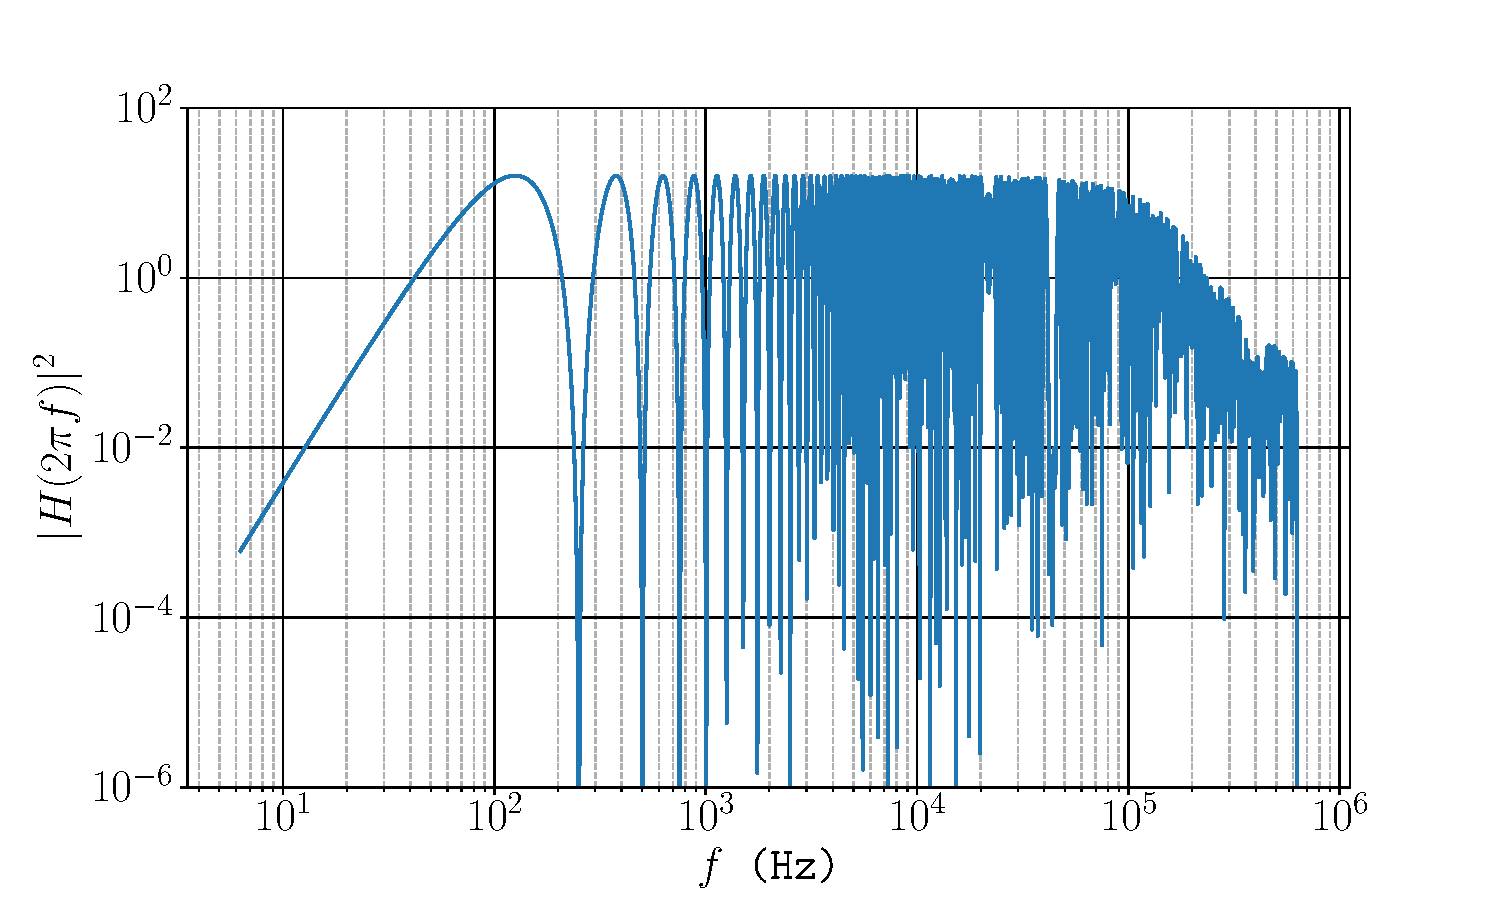
\includegraphics[width=0.7\textwidth]{transfer_func_laser.pdf}
  \caption[Transfer function for laser phase noise.]{Transfer function
  for laser phase noise. Here, the separation between pulses is \(T =
  \)\sivalue{20}{\milli\second} and the \(\pi/2\) pulse time is \(\tau
=\)\sivalue{20}{\micro\second}.}
  \label{fig:transfer_function}
\end{figure}
\par\noindent
The variance of \(\Phi\) is obtained by averaging over \(\psi\)
\begin{equation} 
  \sigma_\Phi^2 = \langle \Phi^2\rangle_\psi = \frac{1}{2} A^2
  |H(\omega)|^2
  \label{eq:var_phi_transfer}
\end{equation} which is related to the phase noise power spectral density
\(S_\phi(\omega)\) by
  \begin{equation}
    \sigma_\Phi^2 = \frac{1}{2}\int_{-\infty}^\infty
    S_\Phi(\omega)|H(\omega)|^2 \frac{\mathrm{d}\omega}{2\pi} =
      \int_0^\infty
    S_\Phi(\omega)|H(\omega)|^2 \frac{\mathrm{d}\omega}{2\pi} 
    \label{eq:phase_noise_psd}
  \end{equation}
Similarly, the Allan variance can be expressed using the transfer
function and the phase noise power spectral density~\cite{Gouet2008}.
The integration time \(\tau_\text{av} = m T_c\) is expressed in multiples
of the experiment cycling time \(T_c\). In the frequency domain, the phase
noise power spectral density is sampled at frequency multiples of
\(f_c = 1/T_c\), so the Allan variance becomes
\begin{equation}
  \sigma^2_\Phi(\tau_\text{av}) = \frac{1}{\tau_\text{av}}
    \sum_{k=1}^\infty |H(2\pi k f_c|)^2S_\phi(2\pi k f_c)
  \label{eq:avar_transfer}
\end{equation}
\par\noindent
The laser phase noise originates from the reference oscillator used in
the phase-locked loop for the M-Squared laser. The phase noise
spectral density and corresponding Allan deviation for increasing
integration time was measured by M-Squared during installation of the
laser system. A plot of the Allan deviation is shown
in~\FigureRef{fig:allan_dev_m2}. At an interferometer pulse
separation of
\(T = \) \sivalue{25}{\milli\second}, the phase noise in the Raman
laser results in an uncertainty in the interferometer phase of
\sivalue{10}{\milli\radian}. 
\begin{figure}[htpb!]
  \centering
  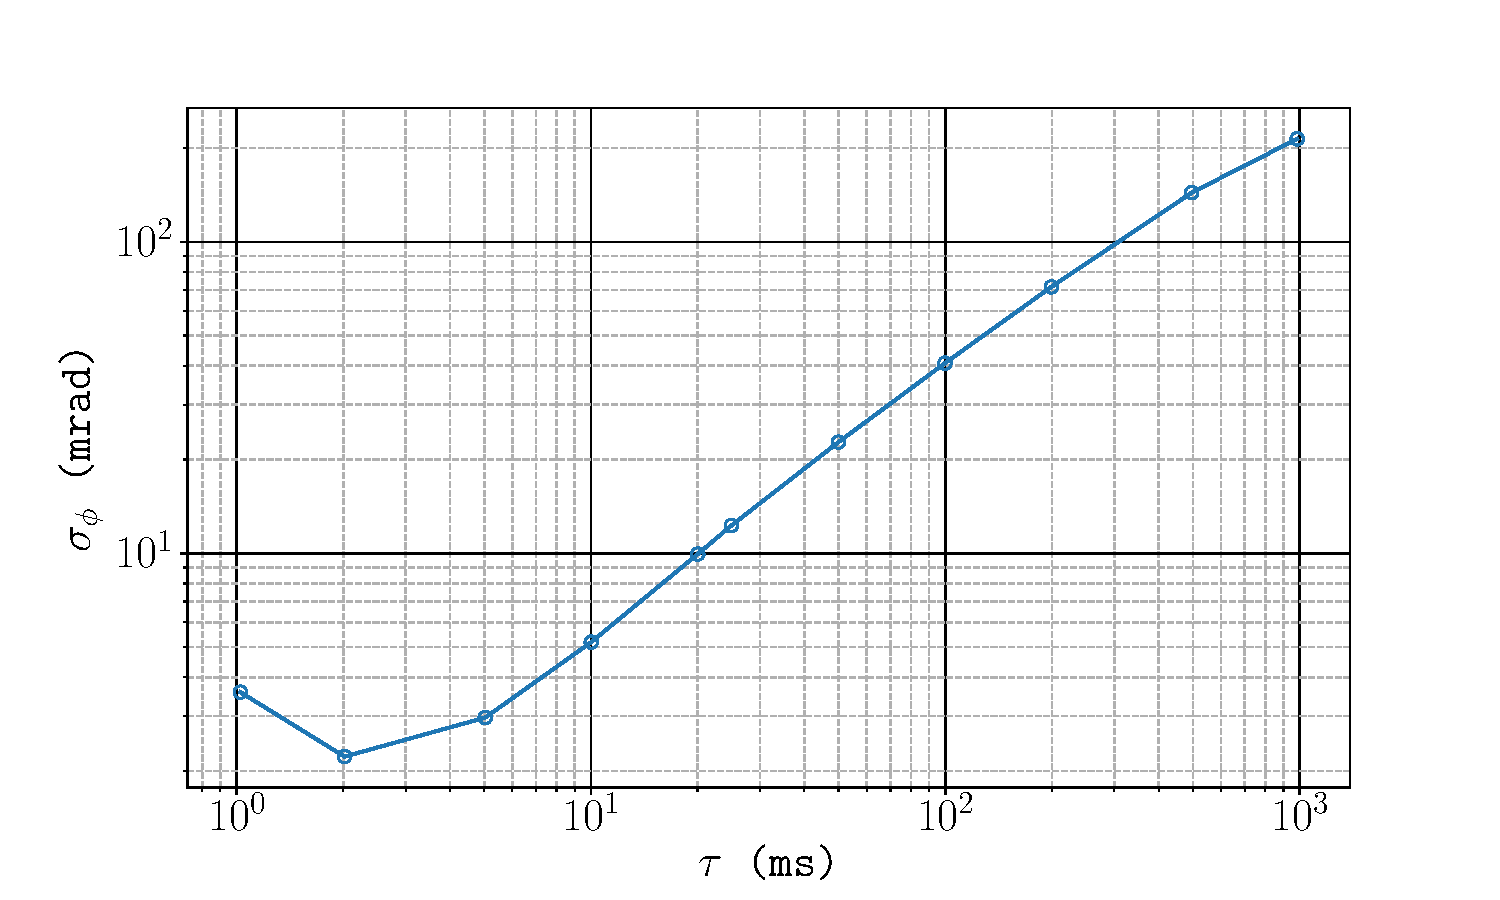
\includegraphics[width=0.7\textwidth]{allan_dev_m2.pdf}
  \caption[Allan deviation of the Raman laser phase difference.]{Allan deviation of the Raman laser phase difference for increasing integration time. Data reproduced from~\cite{M2_manual}.}
  \label{fig:allan_dev_m2}
\end{figure}


\subsection{Vibrations}\label{subsec:vibration_noise}
The phase difference between the two Raman beams depends on the
position of the retro-reflecting mirror. Consequently, this defines a frame of
reference for the position of the atoms during the interferometer. Any
random motion of the mirror, for instance from mechanical vibrations,
introduces a random component to the laser phase~\cite{Vigue2006}. An acceleration of
the mirror modifies the laser phase as follows
\begin{equation}
  \frac{\mathrm{d}^2 \Phi(t)}{\mathrm{d} t^2} = \keff.\textbf{a}(t)
  \label{eq:phase_acc}
\end{equation}
and the sensitivity to accelerations \(g_a\) is given by
\begin{equation}
  \frac{1}{k_\text{eff}} \frac{\mathrm{d}^2 g_a(t)}{\mathrm{d} t^2} =
  g(t) \\
  \label{eq:acc_sens}
\end{equation}
Assuming that the pulse time \(\tau\) is much shorter than the
interferometer pulse separation, \(T\), the acceleration sensitivity
function is approximated by
\begin{equation}
  g_a(t) = \begin{cases}
 -1 & - T < t < 0\\
 1 & 0 < t < T
  \end{cases}
  \label{eq:acc_sens_approx}
\end{equation}
From this, the acceleration transfer function is
\begin{equation}
  |H_a(\omega)|^2 = \frac{k_\text{eff}^2}{\omega^2}|H(\omega)|^2 
  \label{eq:acc_transfer}
\end{equation}
which in the low frequency limit \(\omega \ll \Omega\) is
\begin{equation}
  |H_a(\omega)|^2 = \frac{16 k_\text{eff}^2}{\omega^4}
  \sin\left(\frac{\omega T}{2}\right)^4
  \label{eq:acc_tf_low}
\end{equation}
Equivalent definitions for the variance and Allan variance are
obtained using this and the acceleration noise spectral density
\(S_a(2\pi f)\) as the respective definitions
in~\EquationRef{eq:phase_noise_psd}
and~\EquationRef{eq:avar_transfer}. \FigureRef{fig:transfer_func_acc}
shows the transfer function for
acceleration noise is shown in. The
gain is largest at low frequencies and approximates a second-order
filter at higher frequencies.
\begin{figure}[htpb]
  \centering
  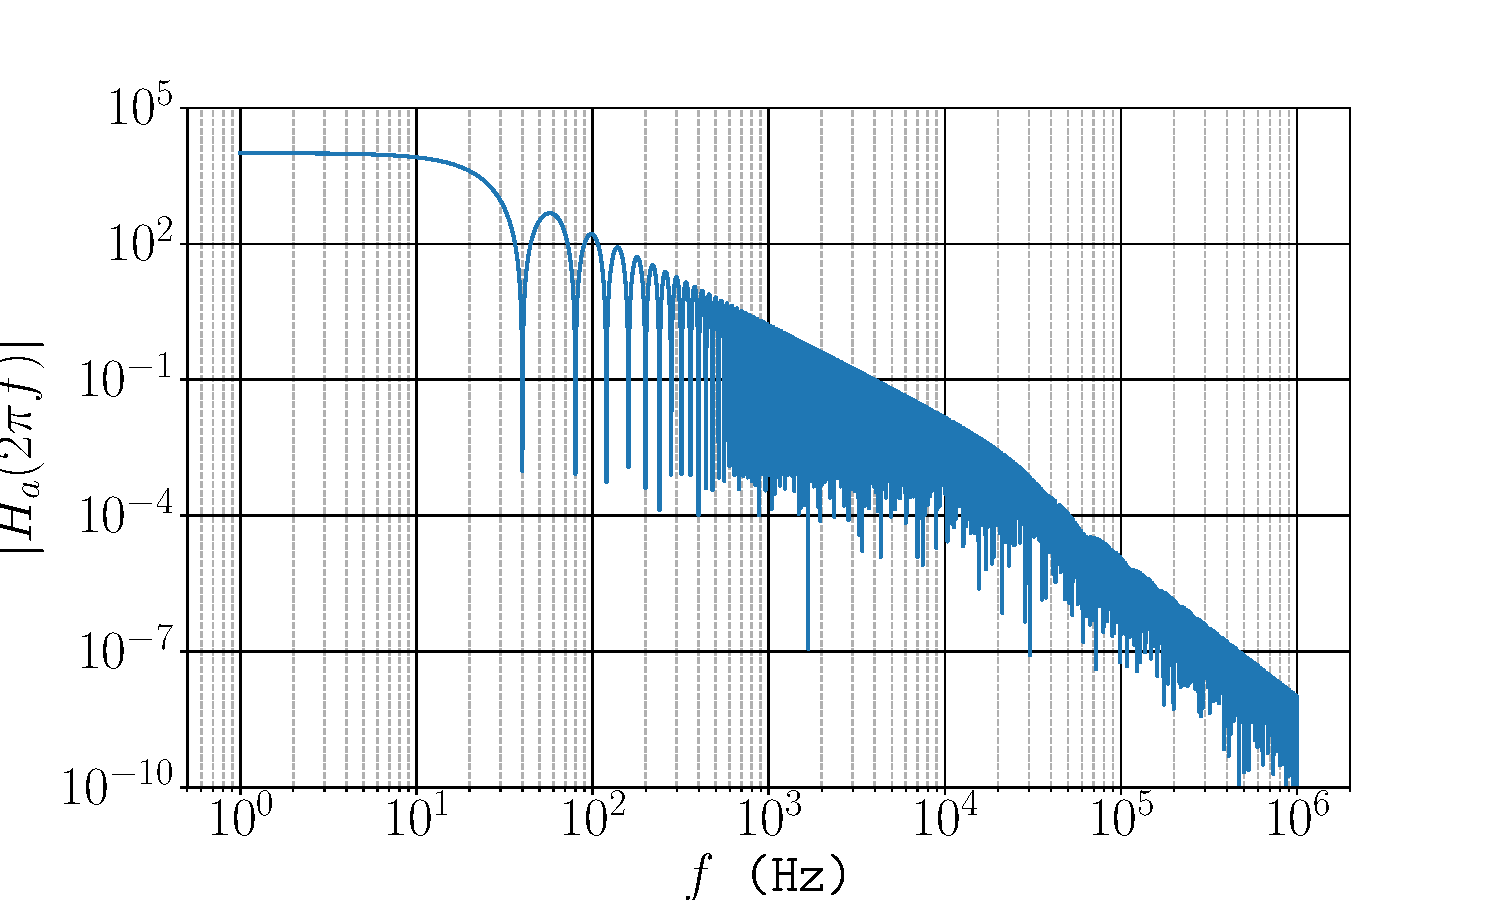
\includegraphics[width=0.7\textwidth]{transfer_func_acc}
  \caption[Acceleration noise transfer function.]{Acceleration noise
  transfer function. The parameters used here are the same as those
previously defined for~\FigureRef{fig:transfer_function}.}
  \label{fig:transfer_func_acc}
\end{figure}
\subsubsection{Measuring the Acceleration Noise Power Spectral Density}
The interferometer phase is most sensitive to low-frequency
vibrations. Acceleration noise at frequencies greater than \(1/2T\)
will mostly average out, contributing little to an overall phase.
Precise measurements of the interferometer phase rely on reducing the
low frequency noise. The vibration of the retro-reflecting mirror is
reduced by passively isolating it from its environment. The
chamber is mounted on a layer of Sorbothane to dissipate
vibrations from the ground. This isolation is enhanced by a
pneumatic suspension system between the optical table and its
supporting legs. 
\par\noindent
\FigureRef{fig:vibration_spectrum} shows a comparison of the acceleration noise spectral density with and
without the pneumatic suspension, measured using
the accelerometer mounted behind the retro-reflecting mirror. The suspension acts as a
low-pass filter and reduces the power within the
10-\sivalue{200}{\hertz} bandwidth, which is aliased into the lower
frequency band. For an interferometer pulse separation of \(T =
\) \sivalue{25}{\ms}, the
vibration phase noise using~\EquationRef{eq:avar_transfer} is \(\sigma_\Phi =\) \sivalue{270}{\milli\radian}. Without
floating the table, this becomes \sivalue{7}{\radian}. This is the dominant
source of phase noise using the current vibration isolation systems.
This phase noise can be reduced using more sophisticated method of damping vibrations, such as an active
isolation system~\cite{Zhou2012}.
\begin{figure}[htpb!]
  \centering
  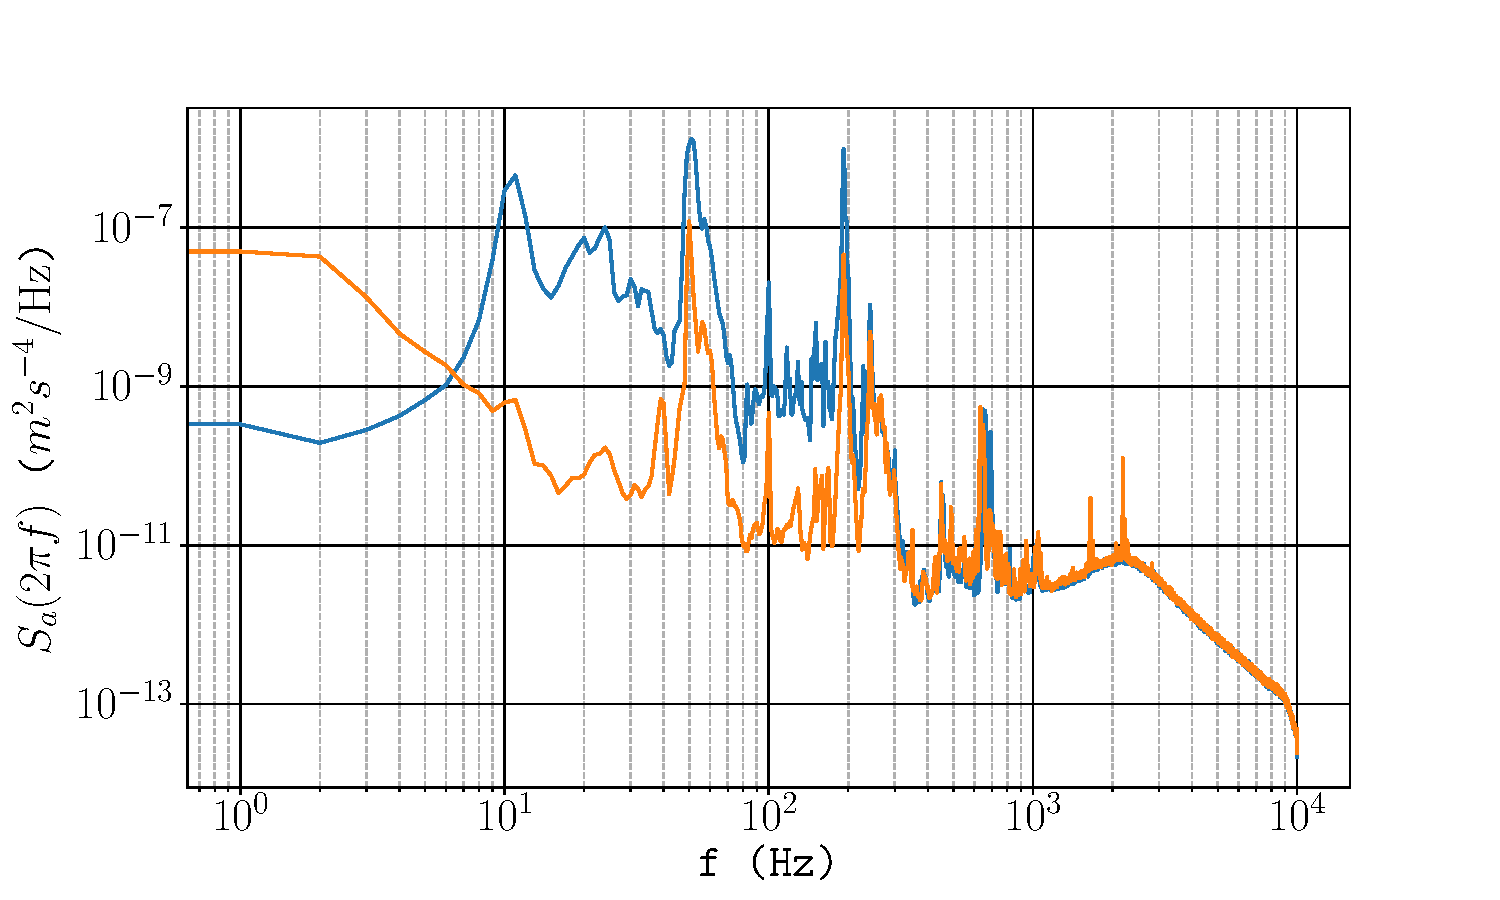
\includegraphics[width=0.7\textwidth]{vibration_spectrum.pdf}
  \caption[Acceleration noise power spectral density.]{Acceleration
  noise power spectral density sampled at a rate of
\sivalue{20}{\kilo\hertz}. The orange curve shows the acceleration
power spectral density using pneumatic suspension to decrease the
coupling of vibrations from the ground to the experiment. For
comparison, the blue curve shows the power spectral density without
this isolation.}
  \label{fig:vibration_spectrum}
\end{figure}
%\subsection{Other Sources of Phase Noise}
%Aside from laser phase noise and vibrations, there are additional effects
%which result in interferometer phase noise. These have not been
%characterised in this experiment as their magnitude is typically much
%smaller than the present vibration phase noise. 
%\begin{itemize}
%  \item \underline{Magnetic field gradients}. The \(\Delta_m = 0\)
%    clock transition has a second-order Zeeman shift of
%    \sivalue{575}{\Hz\gauss\tothe{-2}}. A gradient of magnetic field
%    across the area traversed by the atoms introduces a propagation
%    phase which does not cancel. 
%  \item \underline{Laser intensity noise}.
%\end{itemize}
\subsection{Summary of Identified Noise Sources}\label{subsec:noise_sources}
To conclude this discussion, it is helpful to compare the identified
sources of noise. These are not a complete list of the effects which
reduce the sensitivity to accelerations, but are the most dominant. The
identified sources and their estimated effects on acceleration
measurements are shown in~\TableRef{tab:noise_sources}. The largest
contributor comes from vibrations of the retro-reflecting mirror.
Other noise sources, such as magnetic field gradients, laser intensity
noise and rotations have not yet been characterised. Higher-order
phase shifts due to inertial effects, such as the Coriolis force and
gravity gradients, have been
studied elsewhere\cite{Bongs2006}.
\begin{table}[htpb!]
  \centering
  \begin{tabular}{ccc}
    \toprule
    Noise Source & Signal/Noise & \(\sigma_a\)
    (\sivalue{}{\micro\meter\per\s\squared}) \\
    \midrule
    Projection noise (\num{5e6} atoms) & 2200 & 0.07 \\
    Laser phase noise & 157 & 1 \\
    Technical detector noise & 15 & 10.5 \\
    Vibrations & 5.8 & 26\\
    \bottomrule
  \end{tabular}
  \caption[Comparison of known noise sources.]{Comparison of known noise sources and their effects on
  acceleration measurements. These values are estimated assuming a
separation between pulses of \(T = \)\sivalue{25}{\ms} and a \(\pi/2\)
pulse time of \(\tau = \)\sivalue{20}{\micro\s}.}
  \label{tab:noise_sources}
\end{table}
\section{Measuring Accelerations}\label{sec:atomint_accelerations}
This section presents the techniques used to characterise the atom interferometer
and its sensitivity to accelerations. It begins with a calibration of
the fringe pattern in~\SectionRef{sec:fringe_cal}. Following this, a
method for filtering the effects of vibrations is given
in~\SectionRef{sec:vibration_senstivity}. This section concludes with
a measurement of the Allan variance to determine the long-term
stability in~\SectionRef{subsec:stability}.
\subsection{Fringe Calibration}\label{sec:fringe_cal}
With spatial resolution of the atom cloud, it is possible to resolve
the fringe contrast from a single shot~\cite{Sugarbaker2013}. Of
course, this is not possible using a photodiode, so the fringe
contrast is measured using successive experiment
cycles~\cite{Peters2001}. 
The interferometer phase difference $\Delta \Phi$ is controlled 
by varying the phase difference between the two Raman lasers for the
middle \(\pi\) pulse. Since \(\Delta \Phi = \phi_1 - 2\phi_2
+\phi_3\), varying \(\phi_2\) induces the largest change in
\(\Delta\Phi\). \FigureRef{fig:fringe_examp} shows an interference fringe obtained in this
manner. In this instance, the contrast is \(C = 0.055\) and the mean
probability of detecting in \(\ket{F=2}\) is \(\textnormal{P}_0 =
0.39\).
\begin{figure}[htpb!]
  \centering
  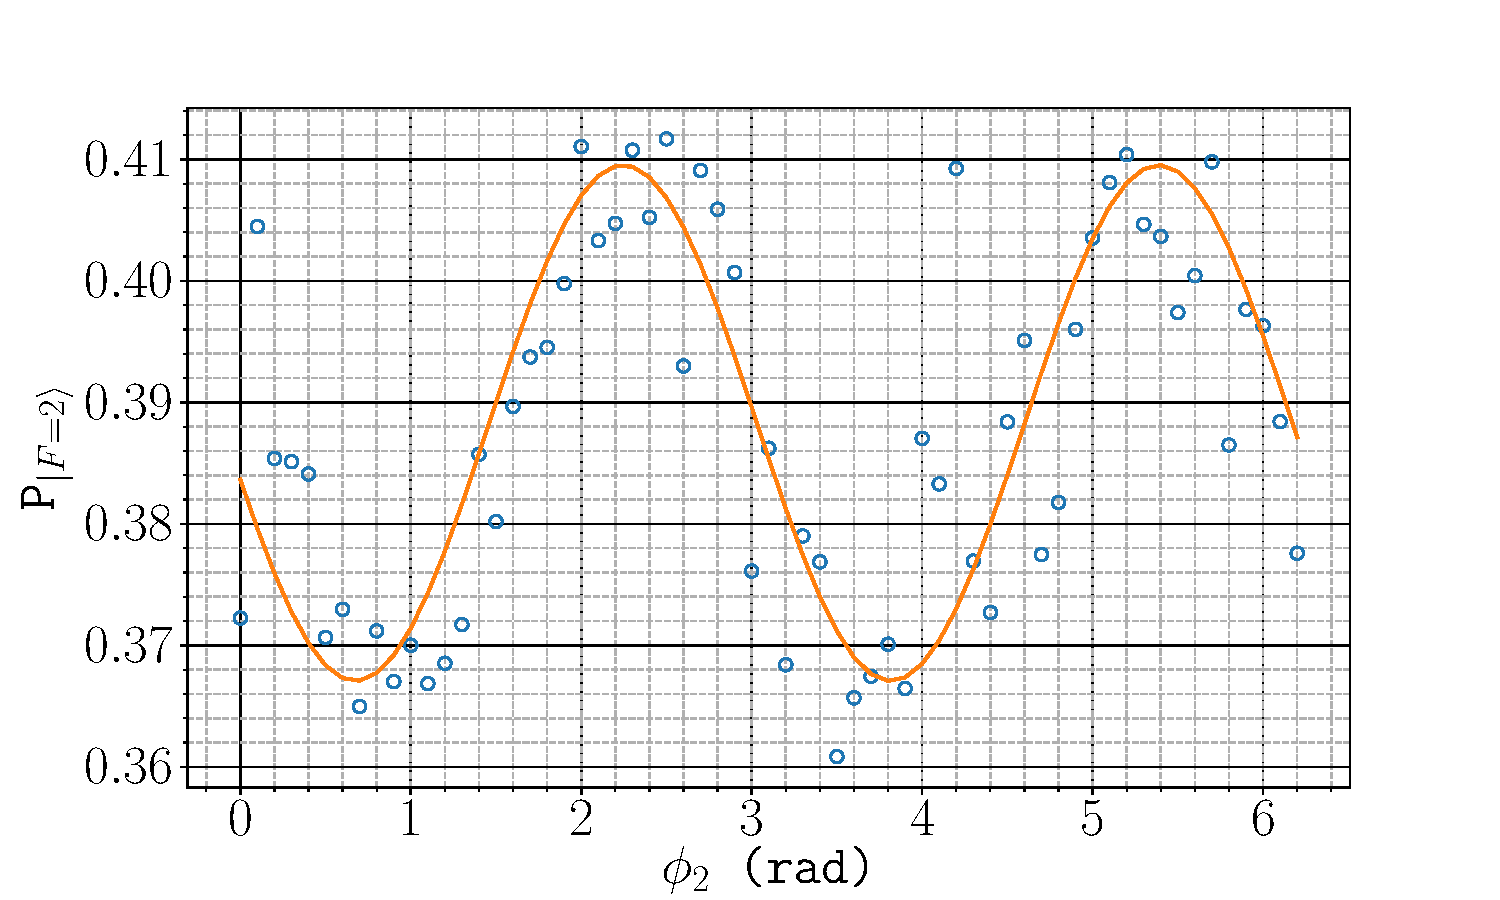
\includegraphics[width=0.7\textwidth]{fringe_examp}
  \caption[Interference fringe for \(T = \)\sivalue{25}{\ms}.]{Interference fringe obtained by varying the phase
    difference of the two Raman lasers during the middle \(\pi\) pulse
    for a pulse separation time of \(T = \)\sivalue{25}{\ms}. The orange
curve is a non-linear least squares fit to the data, giving a contrast
of \(C = 0.055\) and a mean value of \(\textnormal{P}_0 = 0.39\). The
shaded region indicates the 95\% confidence band. }
  \label{fig:fringe_examp}
\end{figure}

\subsection{Correcting for Vibration
Noise}\label{subsec:vibration_sensitivity}
Vibrations of the retro-reflecting mirror are a significant source of
phase noise, which limits the sensitivity of the interferometer to
accelerations. This is particularly apparent when the vibration noise
induces a phase shift of greater than 2\(\pi\) radians. If the
interferometer signal spans multiple fringes, it is not possible to
accurately determine acceleration from the phase shift.
\par\noindent
One method to filter the effects of vibration noise, described in
~\cite{Merlet2009}, uses the MEMS accelerometer to measure the
vibration of the retro-reflecting mirror between the
first and last interferometer pulse. After this time, the phase shift
due to vibrations is given by the following convolution
\begin{equation}
  \phi_\textnormal{vib} =  \keff T^2 K\int_{-T}^{T} g_a (t) V(t)
  \mathrm{d}t = \keff T^2 K
  \widetilde{V}_\textnormal{vib}
  \label{eq:phase_vib}
\end{equation}
where \(V(t)\) is the voltage measured across the output of the MEMS
accelerometer, \(K = \) \sivalue{0.793}{\m\s\tothe{2}\per\V} is the
scaling factor from voltage to acceleration and \(g_a(t)\) is the
acceleration sensitivity function, defined
in~\EquationRef{eq:acc_sens_approx}. Leaving the scaling factor as a
free parameter $\alpha$, the interferometer signal is
fit to the function
\begin{equation}
  \text{P}_{\ket{F=2}} = \text{P}_0 + \frac{C}{2}\sin(\alpha
  \widetilde{V}_\textnormal{vib} + \phi_0)
  \label{eq:fringe_fit_vibration}
\end{equation}
\par\noindent
Common-mode suppression of the vibration phase noise is achieved by
estimating the interferometer phase from the residuals of the fit
to~\EquationRef{eq:fringe_fit_vibration}. If the interferometer phase
as estimated from~\EquationRef{eq:interferometer_phase} is denoted
\(\phi_\textnormal{int}\), then the fit residuals are
\(\phi_\textnormal{res} =  \phi_\textnormal{int} -
\phi_\textnormal{vib}\).
The correlation of the acceleration measured by the MEMS accelerometer
and the interferometer signal is shown
in~\FigureRef{fig:vib_comparison}. The Raman laser phase difference was
initially set so that the interferometer signal was at the mid-point
of the fringe \(\Delta \phi = \pi/2\) before continuously running the
experiment. The vibration noise was increased
by removing the pneumatic suspension of the optical table, which
helps to passively isolate the experiment from external vibrations
that are coupled through the table legs. Without this additional
suppression, the vibration noise is large enough to shift the
interferometer phase by more than \(2\pi\), as indicated
in~\FigureRef{fig:high_vib}. When the table is suspended, the
vibration noise is small enough that the interferometer signal remains
on one side of the fringe.
\begin{figure}[htpb!]
  \centering
  \subfloat[][]{\scalebox{0.5}{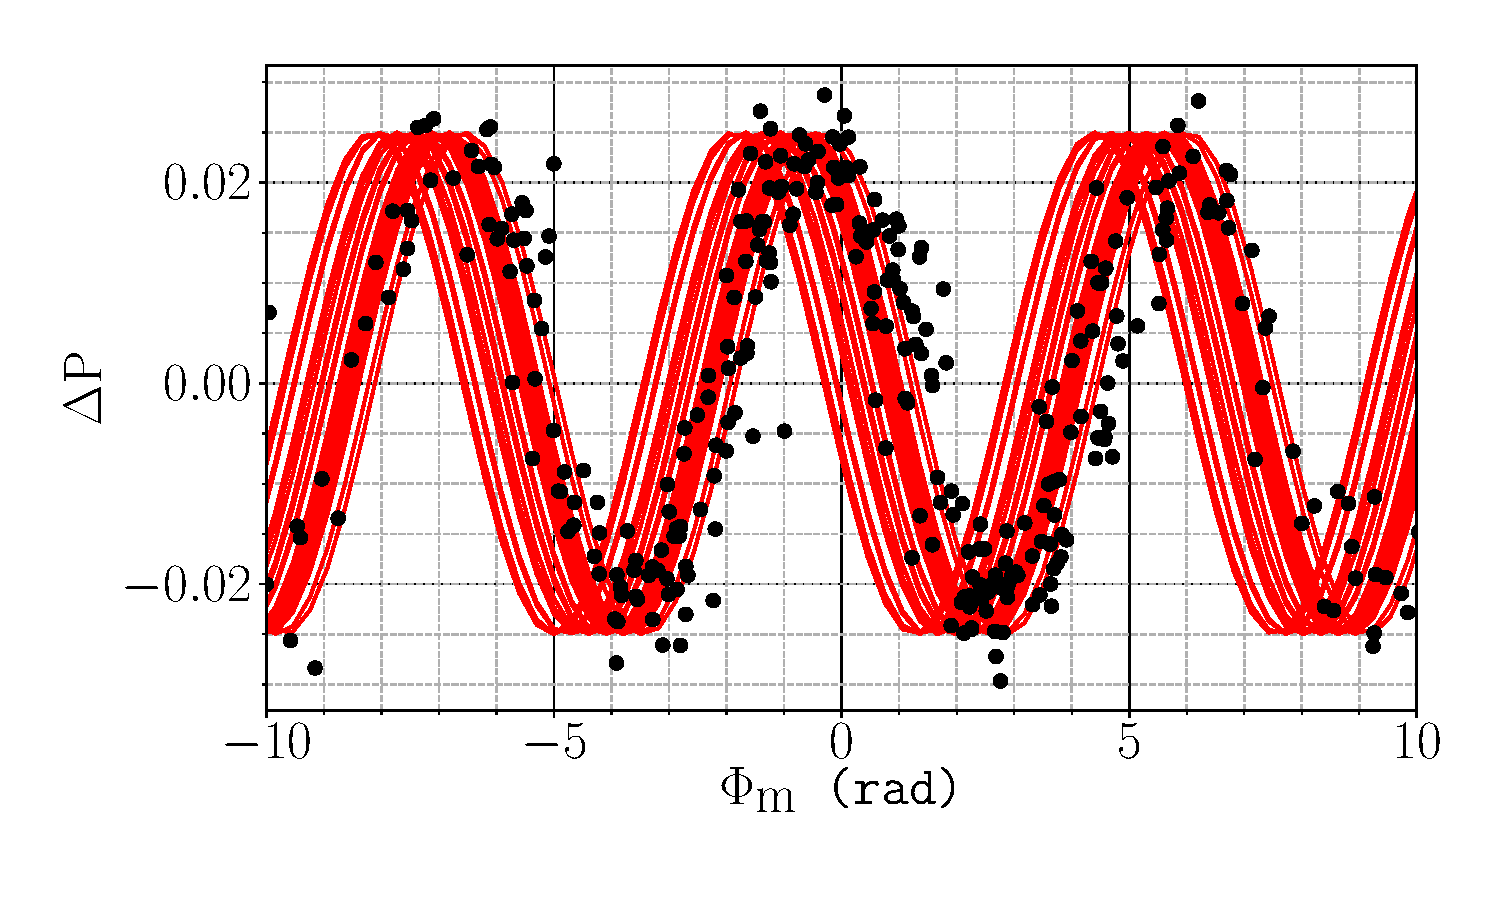
\includegraphics{high_vib}}\label{fig:high_vib}}
    \subfloat[][]{\scalebox{0.5}{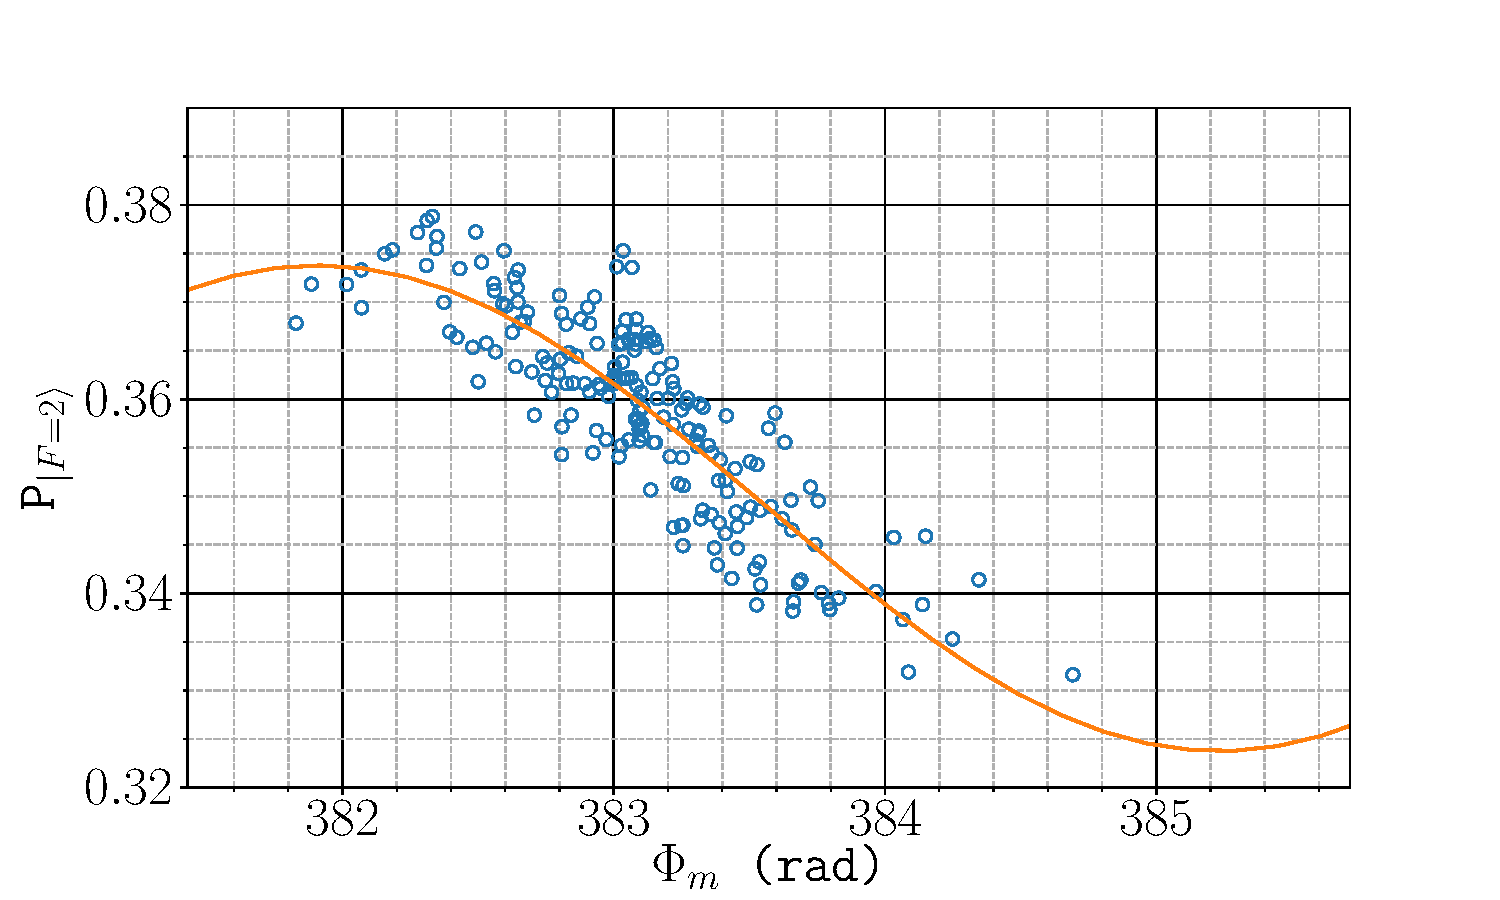
\includegraphics{low_vib}}\label{fig:low_vib}}
  \caption[Comparison of MEMS/Interferometer correlation in a high and
    low vibration
  environments.]{Correlation between acceleration measured by the MEMS
    accelerometer and the interferometer signal. \textbf{(a)} shows
    the correlation measured in high vibration environment, when the
    optical table was not pneumatically suspended. \textbf{(b)} shows
    the reduction in phase noise with this additional vibration
  isolation.}
  \label{fig:vib_comparison}
\end{figure}
\par\noindent
The suppression of the vibration noise can be seen in the distribution
of the estimated acceleration. \FigureRef{fig:vibration_hists} shows
histograms of the acceleration measured by the MEMS and the
interferometer in the low vibration instance
of~\FigureRef{fig:low_vib}. \FigureRef{fig:low_vib_hist_mems_atom} compares the distribution of
the accelerations measured by the MEMS with that of the
interferometer. The noise in the MEMS signal is larger than in the
interferometer -- their respective standard deviations are
$\sigma_a^{(m)} =$ \sivalue{66.8}{\um \s\tothe{-2}} and
$\sigma_a^{(i)} =$ \sivalue{20.8}{\um \s\tothe{-2}}. The MEMS
accelerometer has a higher acceleration bandwidth (\sivalue{20}{\kHz}) than the
interferometer (\sivalue{20}{\Hz}). Consequently, the interferometer
is not sensitive to the high-frequency noise measured by the MEMS
accelerometer. \FigureRef{fig:low_vib_hist_atom_res} compares the acceleration noise
from the interferometer with the acceleration inferred from the fit
residuals
$\phi_\textnormal{res}$. The latter has a standard deviation of
$\sigma_a^{(r)} = $ \sivalue{10.4}{\um \s\tothe{-2}}. This method is
able to filter the effects of vibration from the interferometer
signal. However, the non-linear least squares method assumes that
there is no error in the independent variable
$\tilde{V}_\textnormal{vib}$. This introduces a random
error to $\phi_\textnormal{res}$ from the noise intrinsic to the MEMS
accelerometer. A weighted least-squares fit is
able to account for errors in both variables~\cite{Macdonald1992}. This requires an
accurate estimate of the weights for each measurement of
$\tilde{V}_\textnormal{vib}$ and $\text{P}_{\ket{F=2}}$ to avoid inaccurate
parameter estimates.
\begin{figure}[htpb!]
  \centering
  \subfloat[][]{\scalebox{0.32}{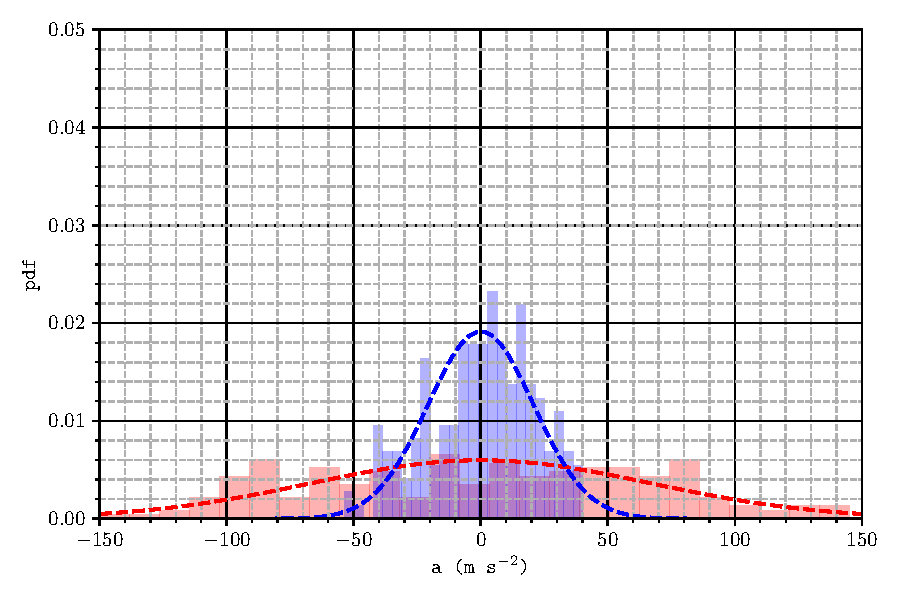
\includegraphics{low_vib_hist_mems_atom}}\label{fig:low_vib_hist_mems_atom}}
    \subfloat[][]{\scalebox{0.32}{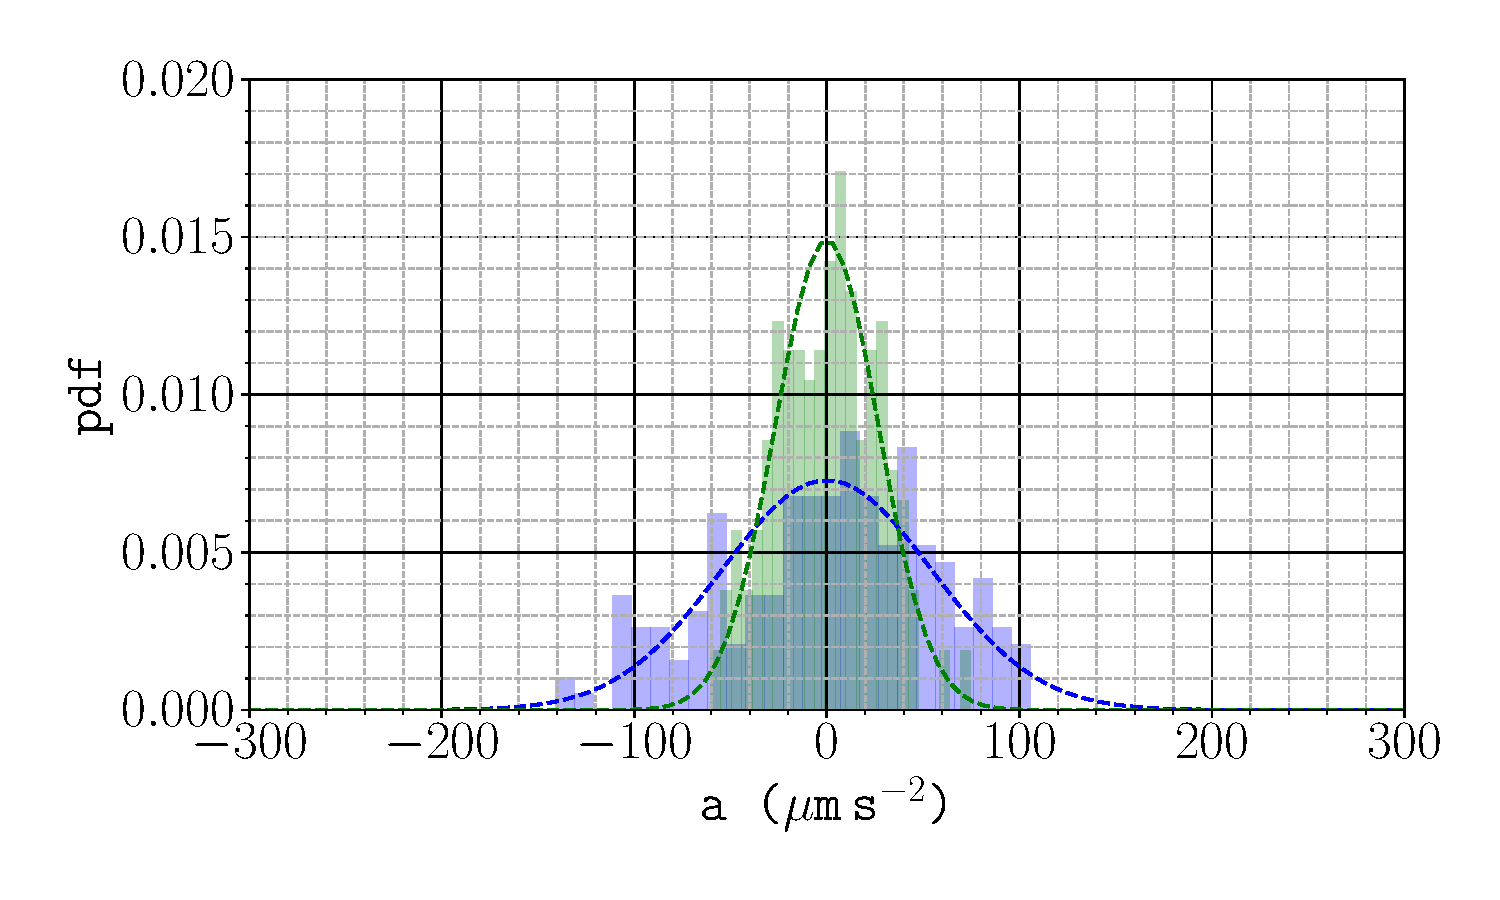
\includegraphics{low_vib_hist_atom_res}}\label{fig:low_vib_hist_atom_res}}
  \caption[Histogram of acceleration noise.]{Histograms of the
    acceleration measured in~\FigureRef{fig:low_vib}. \textbf{(a)} shows
    the distribution of the acceleration measured by the MEMS
    accelerometer (red) and the interferometer (blue). \textbf{(b)} shows
    the distribution after filtering the vibration noise from the
    interferometer signal (green). The dashed lines indicate the
  fitted normal distributions.}
  \label{fig:vibration_hists}
\end{figure}

\subsection{Signal Stability}\label{subsec:stability}	
The stability of the interferometer's sensitivity to accelerations can
be determined from the Allan deviation. A comparison of the
Allan deviation in the presence of high and low vibrations is shown
in~\FigureRef{fig:adev_comparison}. In both instances, the sensitivity
to accelerations is improved by correcting for the vibration-induced
phase. \FigureRef{fig:high_vib_adev} shows the Allan deviation
measured under high vibrations (without floating the optical table).
The Allan deviation has a minimum value
of around \sivalue{3e-6}{\m\s\tothe{-2}} after integrating for
\sivalue{35}{\s}. This is a bias instability, i.e. fluctuations in
the bias. This value is obtained by subtracting the vibration
phase, estimated from the MEMS accelerometer, from the interferometer
phase. There is additional noise in the MEMS
accelerometer which leads to this bias instability. At short
integration times, the Allan deviation has a $\tau^{-1}$
dependence. It is likely that this arises from additional low
frequency noise from the MEMS signal~\cite{Meunier2015, Fang2016}. This is
well-correlated between successive measurements, where the dead time
between them means that full dynamics of the system are not captured. In the context of
atomic clocks, this is referred to as the Dick effect~\cite{Dick1990}.  
\par\noindent
\FigureRef{fig:low_vib_adev} shows the Allan devation in the case of
smaller vibrations. In contrast to the previous case, the signal
remains stable for a longer period of time. The Allan deviation
is proportional to \(\tau^{-1/2}\), which is characteristic of
uncorrelated white phase noise. At longer integration times, the
small number of samples introduces a large uncertainty on the Allan
deviation. For times up to \sivalue{100}{\s}, 
the sensitivity of the signal is not limited by bias
instability. 
\begin{figure}[htpb!]
  \centering
  \subfloat[][]{\scalebox{0.3}{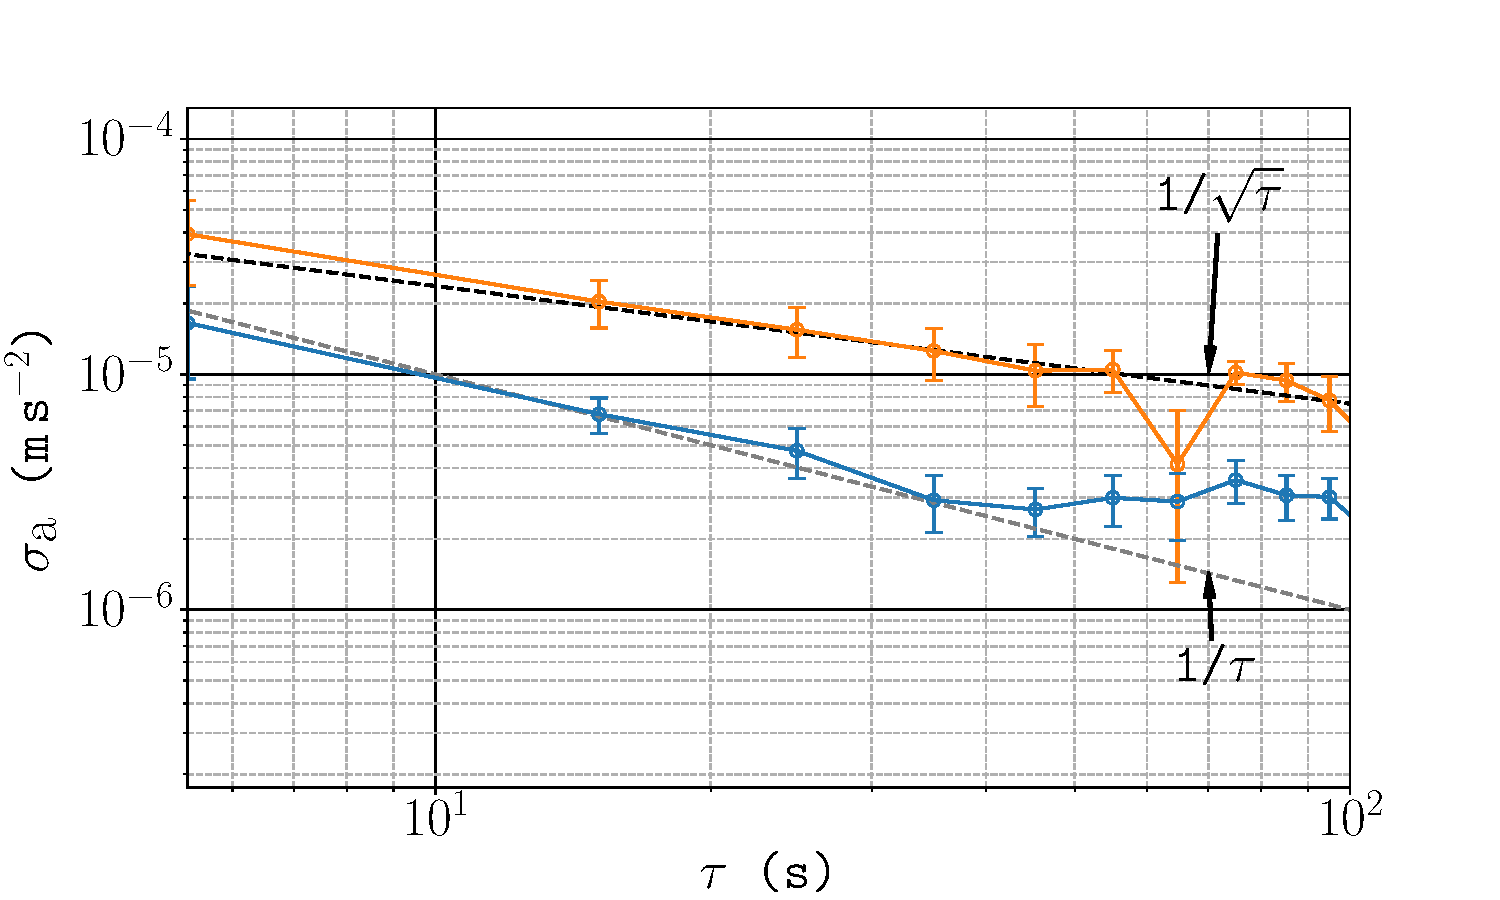
\includegraphics{high_vib_adev}}\label{fig:high_vib_adev}}
    \subfloat[][]{\scalebox{0.3}{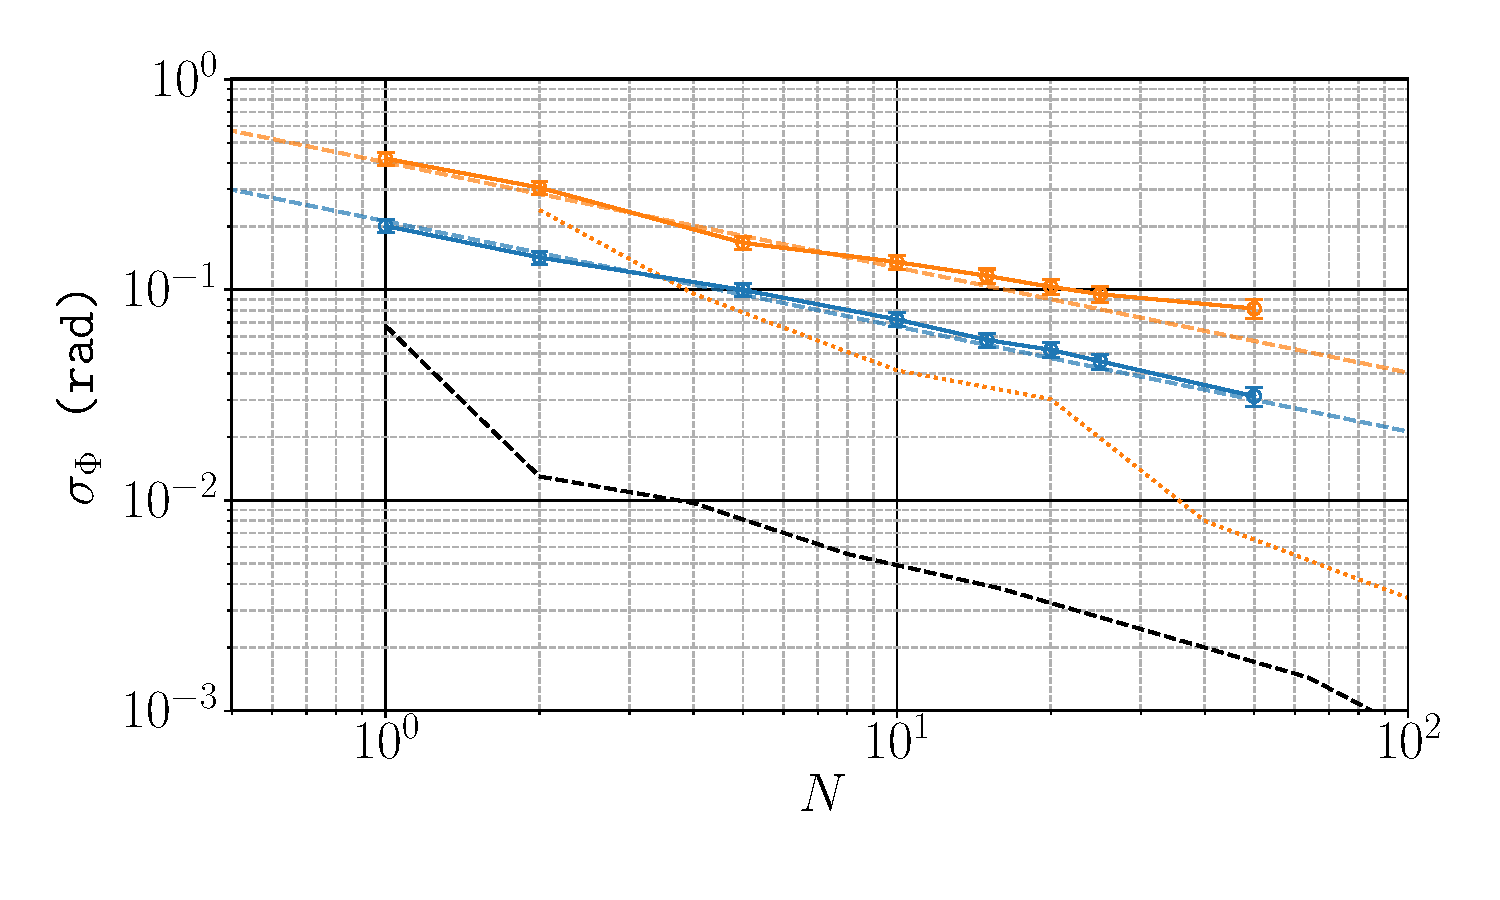
\includegraphics{low_vib_adev}}\label{fig:low_vib_adev}}
  \caption[Comparison of Allan deviation in a high and
    low vibration
  environment.]{Allan deviation of the estimated acceleration using
    the interferometer signal. In each plot the orange curve
    represents the sensitivity to accelerations without subtracting
    the vibration induced phase, and the blue curve shows the
    sensitivity after subtracting this. 
    As in~\FigureRef{fig:vib_comparison}, \textbf{(a)} shows
    the sensitivity in a high vibration environment, and
    \textbf{(b)} shows it after reducing the level of vibration.}
  \label{fig:adev_comparison}
\end{figure}

\section{Conclusion}
This chapter has described the methods used to observe matter-wave
interference. It has presented a description of the Raman laser system
and the scheme used to infer the population in each internal state. 
The light pulses used to drive Raman
transitions were subsequently presented, to emphasise the effect of
a light shift and background atoms on the interferometer. A further
discussion of identified noise sources showed that vibrations are the
largest contributor. The interference between two states was
characterised
